\PassOptionsToPackage{dvipsnames}{xcolor}
\documentclass{beamer}  % handout to collapse the PAUSES
\usepackage[utf8]{inputenc}
\usepackage{mathtools}
\usepackage{amsmath,amsfonts,amssymb,amsthm,bm}
\usepackage{stmaryrd}
\usepackage{xfrac}
\usepackage{nccmath}
\usepackage{hyperref}
\usepackage{svg}
\usepackage{graphicx}
\usepackage{cancel}
\usepackage{physics}
\usepackage{hyperref}
\usepackage{subcaption}
\usepackage{tikz}
\usetikzlibrary{
  calc, patterns, angles, quotes,
  decorations.pathmorphing, decorations.markings, decorations.text,
  shapes, shapes.multipart,backgrounds,arrows.meta
}

\usepackage{animate}
\usepackage{multimedia}
% \usepackage{media9}

\usepackage{empheq}
\usepackage[many]{tcolorbox}
\newtcolorbox{empheqboxed}[1][]{
  colback=gray!20,
  colframe=white,
  width=\textwidth,
  sharpish corners,
  top=4pt, % default value 2mm
  bottom=3pt,
  %after=,% <----- remove the default \par
}

\newcommand{\xx}{\mathbf{x}}
\newcommand{\vv}{\mathbf{v}}
\newcommand{\uu}{\mathbf{u}}
\newcommand{\ff}{\mathbf{f}}
\newcommand{\gam}{\boldsymbol{\dot \gamma}}
\newcommand{\nn}{\mathbf{\hat n}}

\DeclareMathOperator*{\argmin}{arg\,min}
\DeclareMathOperator*{\minimize}{minimize}

% \usetheme{Boadilla}
% \usecolortheme{default}
% %\setbeamertemplate{sections/subsections in toc}[sections numbered]
% \useinnertheme{rectangles} % adds squared bullets to TOC

\usetheme{CambridgeUS}
\useoutertheme{infolines} % Alternatively: miniframes, infolines, split
\useinnertheme{rectangles}

\definecolor{UBCblue}{rgb}{0.04706, 0.13725, 0.26667} % UBC Blue (primary)
\definecolor{UBCgrey}{rgb}{0.3686, 0.5255, 0.6235} % UBC Grey (secondary)

\setbeamercolor{palette primary}{bg=UBCblue,fg=white}
\setbeamercolor{palette secondary}{bg=UBCblue,fg=white}
\setbeamercolor{palette tertiary}{bg=UBCblue,fg=white}
\setbeamercolor{palette quaternary}{bg=UBCblue,fg=white}
\setbeamercolor{structure}{fg=UBCblue} % itemize, enumerate, etc
\setbeamercolor{section in toc}{fg=UBCblue} % TOC sections
\setbeamercolor{titlelike}{fg=UBCblue} % TOC sections
\setbeamercolor{frametitle}{fg=UBCblue} % TOC sections


% Override palette coloring with secondary
\setbeamercolor{subsection in head/foot}{bg=UBCgrey,fg=white}

\setbeamertemplate{itemize item}[triangle]
\setbeamertemplate{enumerate item}[circle]
%\setbeamercolor*{enumerate item}{fg=red}
%\setbeamercolor*{enumerate subitem}{fg=red}
%\setbeamercolor*{enumerate subsubitem}{fg=red}
%\setbeamercolor*{itemize item}{fg=red}
%\setbeamercolor*{itemize subitem}{fg=red}
%\setbeamercolor*{itemize subsubitem}{fg=red}
%\setbeamercovered{transparent}

%------------------------------------------------------------

%\title[Queues] {Queues}
%\subtitle{Vincent Degrooff  Christophe Heneffe  Guillaume Lejeune}

\title[Yield stress fluids]{Numerical simulation of yield stress fluid flows}
\subtitle{Master's thesis}
\titlegraphic{
    \includesvg[height=0.7cm]{./UCLouvain_logo.svg}
    \hspace*{2cm}~
    \includesvg[height=0.9cm]{./Logo_EPL.svg}
}
\author[Vincent Degrooff]{
    Vincent Degrooff
    %Promotor: Jean-François Remacle
}
\date[26 June 2023]{}
\institute[]{\normalsize Promotor: Jean-François Remacle}


%------------------------------------------------------------
%The next block of commands puts the table of contents at the 
%beginning of each section and highlights the current section:

\AtBeginSection[]
{
  \begin{frame}
    \frametitle{Table of Contents}
    \tableofcontents[currentsection]
  \end{frame}
}
%------------------------------------------------------------


\begin{document}

\frame{\titlepage}


\begin{frame}
\frametitle{Table of Contents}
\tableofcontents
\end{frame}

%---------------------------------------------------------

\section{What is a yield stress fluid ?}

\begin{frame}{}
    \begin{columns}
        \begin{column}{.45\textwidth}
            \begin{itemize}
                \item Domain $\Omega$
                \item Position vector $\xx \in \Omega$
                \item Velocity field $\vv(\xx)$
                \item Fluid undergoes stress $\boldsymbol{\sigma} = -p\mathbf{I} + \boldsymbol\tau$
                \item Need to relate $\boldsymbol\tau$ to $\vv$
            \end{itemize}
        \end{column}
        \begin{column}{.45\textwidth}
            \begin{figure}
                \centering
                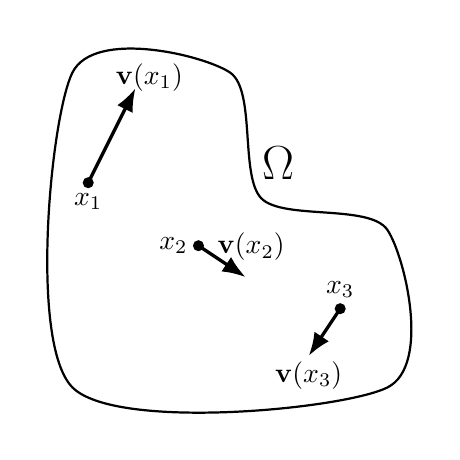
\begin{tikzpicture} [line width=1.2, scale=2 ]
                    \coordinate (0) at (0, 0);
                    \coordinate (c1) at (2, 0);
                    \coordinate (c2) at (2, 1);
                    \coordinate (c3) at (1.2, 1.2);
                    \coordinate (c4) at (1, 2);
                    \coordinate (c5) at (0, 2);
                    \draw[black, thick] plot [smooth cycle] coordinates {(0) (c1) (c2) (c3) (c4) (c5)};
                    %\draw[black, ->] (1.1, 0.5) -- (1., 0.2);
                    \coordinate (x1) at (0.1, 1.3);
                    \coordinate (x2) at (0.8, 0.9);
                    \coordinate (x3) at (1.7, 0.5);
                    \node[anchor=north] at (x1) {$x_1$};
                    \node[anchor=east] at (x2) {$x_2$};
                    \node[anchor=south] at (x3) {$x_3$};
                    \fill (x1) circle[radius=1pt];
                    \fill (x2) circle[radius=1pt];
                    \fill (x3) circle[radius=1pt];
                    \draw[-Latex] (x1) -- (0.4, 1.9) node[right=5pt,above=-5pt] {$\vv(x_1)$};
                    \draw[-Latex] (x2) -- (1.1, 0.7) node[right=2pt,above=2pt] {$\vv(x_2)$};
                    \draw[-Latex] (x3) -- (1.5, 0.2) node[left=0pt,below=-2pt] {$\vv(x_3)$};
                    \node[right=6pt, above=3pt] at (c3){\LARGE $\Omega$};
                \end{tikzpicture}
            \end{figure}
        \end{column}
    \end{columns}
\end{frame}

\begin{frame}{Velocity modes}
    \begin{align*}
        \nabla \vv &= {\color{gray!50}\mathbf{D}_s} + \mathbf{D}_d + \mathbf{W}\\
        \only<2>{\boldsymbol\tau &= \mu \; 2 \mathbf{D}_d \qquad \text{(Newtonian fluids)}}
        % \only<2>{\text{Newton}\qquad \boldsymbol\tau &= \mu \; 2 \mathbf{D}_d = \mu \gam = \mu (\nabla \vv + \nabla \vv^\top - {\color{gray!50} 2 \Tr \nabla \vv})}
    \end{align*}
    \begin{figure}
        \centering
        \begin{subfigure}[t]{0.32\textwidth}
            %\movie[width=\textwidth, height=\textwidth, showcontrols, loop]{} {../anim/kinematics_stretch.mp4}
            \animategraphics[autoplay,loop,width=\textwidth]{20}{../anim/kinematics_stretch/frame}{1}{51}    
            \caption{\color{gray!50} expansion}
        \end{subfigure}
        \begin{subfigure}[t]{0.32\textwidth}
            %\movie[width=\textwidth, height=\textwidth, showcontrols, loop]{} {../anim/kinematics_shear.mp4}
            \animategraphics[autoplay,loop,width=\textwidth]{20}{../anim/kinematics_shear/frame}{1}{51}    
            \caption{shear}
        \end{subfigure}
        \begin{subfigure}[t]{0.32\textwidth}
            %\movie[width=\textwidth, height=\textwidth, showcontrols, loop]{} {../anim/kinematics_rotation.mp4}
            \animategraphics[autoplay,loop,width=\textwidth]{20}{../anim/kinematics_rotation/frame}{1}{51}
            \caption{rotation}
        \end{subfigure}
    \end{figure}
\end{frame}

% \begin{frame}{Newtonian fluids}
%     \begin{itemize}
%         \item Need relation between kinematic ($\vv$) and dynamic ($\boldsymbol{\tau}$) quantities.
%         \item Newton assumed that strain-rate $\gamma$ is proportional to shear stress $\tau$, through viscosity $\mu$.
%     \end{itemize}

%     \begin{columns} % align columns
%         \begin{column}{.48\textwidth}
%             %\color{red}\rule{\linewidth}{4pt}
%             \begin{equation*}
%                 \begin{aligned}
%                     \dot\gamma &= \pdv{u}{y}\\
%                     \tau &= \mu \dot\gamma
%                 \end{aligned}
%             \end{equation*}
%         \end{column}%
%         \hfill%
%         \begin{column}{.48\textwidth}
%             %\color{blue}\rule{\linewidth}{4pt}
%             \begin{figure}
%                 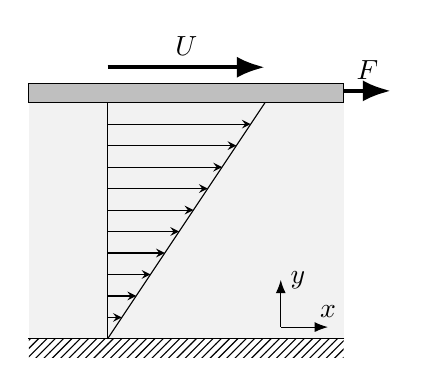
\begin{tikzpicture}
  %[background rectangle/.style={fill=gray!15}, show background rectangle]
  \tikzstyle{ground1}=[draw, fill=gray!50, minimum width=0.75cm,minimum height=0.2cm]
  \tikzstyle{ground2}=[fill,pattern=north east lines,draw=none, minimum width=0.75cm,minimum height=0.2cm]

  \pgfmathsetmacro{\h}{1.5}
  \pgfmathsetmacro{\l}{2.}
  \pgfmathsetmacro{\u}{\l}
  \pgfmathsetmacro{\n}{10}

  \fill [color=black, fill=gray!10!white] (-0.5*\l, -\h) rectangle (1.5*\l, \h);

  \node (wall_up) [ground1, minimum width=2*\l cm, yshift=\h cm, anchor=south, xshift=0.5*\l cm] {};
  %\draw [line width=1mm] (wall_up.south east) -- (wall_up.south west);

  \node (wall_down) [ground2, minimum width=2*\l cm, yshift=-\h cm, anchor=north, xshift=0.5*\l cm] {};
  \draw (wall_down.north east) -- (wall_down.north west);

  \draw (0., -\h) -- (\u, \h);
  \draw (0., -\h) -- (0., \h);
  \foreach \i in {1,...,\n} {
    \draw[-stealth] (0., {\h * (2.*\i/(\n+1) - 1)}) -- ({\u * \i/(\n+1)}, {\h * (2.*\i/(\n+1) - 1)});
  }
  \draw[-Latex, ultra thick] (0.,1.3*\h) -- (\u, 1.3*\h) node [midway, above] {$U$};
  \draw[-Latex, ultra thick] (1.5*\l,1.1*\h) -- (1.8*\l, 1.1*\h) node [midway, above] {$F$};

  \draw[-Latex] (1.1*\l, -0.9*\h) -- (1.1*\l + 0.4*\h, -0.9*\h) node[anchor=south] {$x$};
  \draw[-Latex] (1.1*\l, -0.9*\h) -- (1.1*\l, -0.9*\h + 0.4*\h) node[anchor=west] {$y$};

\end{tikzpicture}

%             \end{figure}
%         \end{column}%
%     \end{columns}
% \end{frame}

% \begin{frame}{Newtonian fluids}
%     \begin{itemize}
%         \item For general flows: $\vv(\xx)$, $\vv$ and $\xx \in \mathbb{R}^3$
%     \end{itemize}

%     \begin{equation*}
%         \begin{alignedat}{2}
%             \nabla \vv &= \pdv{v_i}{x_j} \mathbf{\hat e}_i \mathbf{\hat e}_j\\
%             \mathbf{D} &= \textrm{sym}(\nabla \vv) &&= (\nabla \vv + \nabla^\top \vv)/2 = \boldsymbol{\dot\gamma} / 2\\
%             \mathbf{W} &= \textrm{antisym}(\nabla \vv) &&= (\nabla \vv - \nabla^\top \vv)/2\\
%             %\boldsymbol\tau &= \mu \boldsymbol{\dot\gamma}
%         \end{alignedat}
%             \end{equation*}
%     \begin{empheqboxed}
%         \begin{equation*}
%             \boldsymbol\tau = \mu \boldsymbol{\dot \gamma}
%         \end{equation*}
%     \end{empheqboxed}
% \end{frame}


% \begin{frame}{Strain tensor - stretching}
%     \begin{figure}
%         \centering
%         %autostart,loop,continue,start=0s,duration=60s 
%         \movie[width=0.7\textheight, height=0.7\textheight, showcontrols]{} {../anim/kinematics_stretch.mp4}
%         % \animategraphics[loop,width=6cm]{40}{../anim/kinematics_rotation/frame}{1}{51}
%     \end{figure}
%     % \includemedia[
%     %     width=0.4\linewidth,
%     %     height=0.3\linewidth,
%     %     activate=pageopen,
%     %     addresource=../anim/kinematics_rotation.mp4,
%     %     flashvars={source=../anim/kinematics_rotation.mp4}
%     % ]{}{VPlayer.swf}
% \end{frame}

% \begin{frame}{Strain tensor - shearing}
%     \begin{figure}
%         \centering
%         \movie[width=0.7\textheight, height=0.7\textheight, showcontrols]{} {../anim/kinematics_shear.mp4}
%         % \animategraphics[loop,width=6cm]{40}{../anim/kinematics_shear/frame}{1}{51}
%     \end{figure}
% \end{frame}

% \begin{frame}{Spin tensor - rotation}
%     \begin{figure}
%         \centering
%         \movie[width=0.7\textheight, height=0.7\textheight, showcontrols]{} {../anim/kinematics_rotation.mp4}
%         % \animategraphics[loop,width=6cm]{40}{../anim/kinematics_rotation/frame}{1}{51}
%     \end{figure}
% \end{frame}

\begin{frame}{Flow curve}
    \begin{figure}
        \centering
        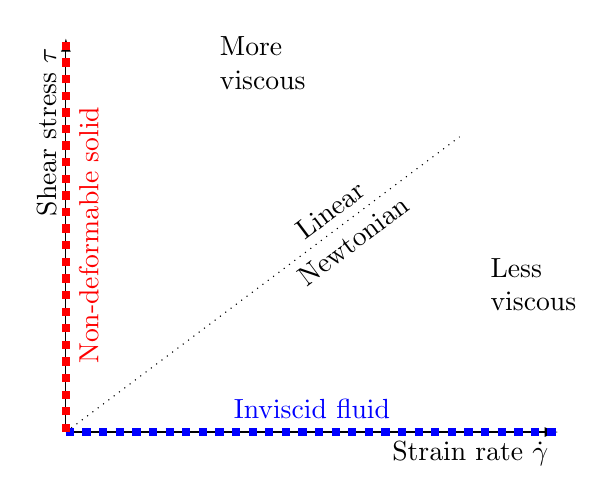
\begin{tikzpicture}[scale=1.25]
            \coordinate (o) at (0., 0.);
            \draw[-Latex] (o) -- (5., 0.) node[anchor=north east] {Strain rate $\dot \gamma$};
            \draw[-Latex] (o) -- (0., 4.) node[anchor=south east, rotate=90] {Shear stress $\tau$};
            \draw[dotted] (o) -- (4., 3.) node [pos=0.7, above, sloped] {Linear} node [pos=0.7,below,sloped] {Newtonian};
            \node[align=left] at (4.75, 1.5) {Less\\viscous};
            \node[align=left] at (2., 3.75) {More\\viscous};
            \draw[line width=1mm, dashed, Blue] (0., 0.) -- (5., 0.) node[midway, above] {Inviscid fluid};
            \draw[line width=1mm, dashed, Red] (0., 0.) -- (0., 4.) node[midway, below, rotate=90] {Non-deformable solid};
        \end{tikzpicture}
        %\caption{Flow curve}
    \end{figure}
\end{frame}

\begin{frame}{Non-Newtonian fluids}
    \begin{itemize}
        \item Generalized Newtonian model
        \begin{equation*}
            \boldsymbol{\tau} = \mu(\dot \gamma, T) \;\boldsymbol{\dot \gamma} \qquad \text{where} \quad
            \begin{cases}
                \gam = 2 \mathbf{D} = \nabla \vv + \nabla \vv^\top\\
                \dot \gamma = \|\boldsymbol{\dot \gamma}\|_F = \sqrt{\Tr(\boldsymbol{\dot \gamma} \cdot \boldsymbol{\dot \gamma})}
            \end{cases}
        \end{equation*}
        \pause
        \item Power-law model
        \begin{equation*}
            \boldsymbol\tau = (K \dot \gamma^n) \; \gam
        \end{equation*}
        \pause
        \item Herschel-Bulkley model (Bingham with $n=1$)
        \begin{align*}
            \gam &= 0 & \text{if} \quad \tau < \tau_0\\
            \boldsymbol\tau &= \left(K \dot \gamma^{n-1} + \frac{\tau_0}{\dot \gamma}\right) \gam & \text{if} \quad \tau \geq \tau_0\\
        \end{align*}
    \end{itemize}    
\end{frame}

\begin{frame}{Non-Newtonian fluids}
    \begin{figure}
        \centering
        \includesvg[width=\textwidth]{../figures/fluid_classification_slide.svg}
    \end{figure}
\end{frame}

%---------------------------------------------------------

\section{Why do we study it ?}

\begin{frame}{Solid-Liquid subdomains}
    \begin{figure}
        \centering
        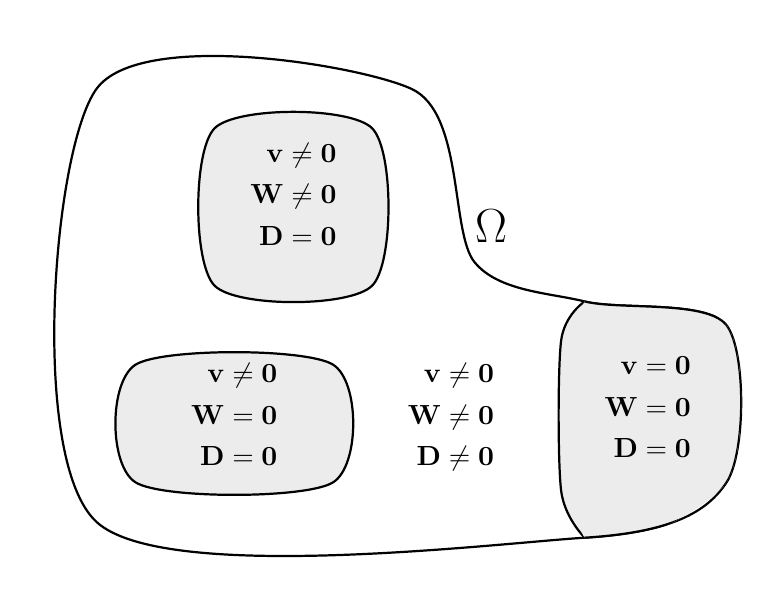
\begin{tikzpicture} [line width=1.2, scale=2 ]
            \coordinate (0) at (0, -0.25);
            \coordinate (x1) at (3.1, -0.35);
            \coordinate (c1) at (4, 0);
            \coordinate (c2) at (4, 1);
            \coordinate (x2) at (3.1, 1.15);
            \coordinate (c3) at (2.4, 1.4);
            \coordinate (c4) at (2, 2.5);
            \coordinate (c5) at (0, 2.5);
            \node[right=6pt, above=3pt] at (c3){\LARGE $\Omega$};
            \draw[black, thick] plot [smooth cycle] coordinates {(0) (x1) (c1) (c2) (x2) (c3) (c4) (c5)};
            \node[anchor=north] at (2.25, 0.85) {
                $\begin{aligned}
                    \vv &\neq \mathbf{0}\\
                    \mathbf{W} &\neq \mathbf{0}\\
                    \mathbf{D} &\neq \mathbf{0}
                \end{aligned}$
            };
            \pause
            \draw[black, thick, fill=gray!15] plot [smooth] coordinates {(x1) (2.95, -0.05) (2.95, 0.9) (x2)};
            \begin{scope}
                \clip plot [smooth cycle] coordinates {(x1) (c1) (c2) (x2)};
                \draw[fill=gray!15, thick] plot [smooth cycle] coordinates {(0) (x1) (c1) (c2) (x2) (c3) (c4) (c5)};
            \end{scope}
            \node[anchor=north] at (3.5, 0.9) {
                $\begin{aligned}
                    \vv &= \mathbf{0}\\
                    \mathbf{W} &= \mathbf{0}\\
                    \mathbf{D} &= \mathbf{0}
                \end{aligned}$
            };
            \pause
            \draw[black, thick, fill=gray!15] plot [smooth cycle] coordinates {(0.25, 0.) (1.5, 0.) (1.5, 0.75) (0.25, 0.75)};
            \node[anchor=north] at (0.875, 0.85) {
                $\begin{aligned}
                    \vv &\neq \mathbf{0}\\
                    \mathbf{W} &= \mathbf{0}\\
                    \mathbf{D} &= \mathbf{0}
                \end{aligned}$
            };
            \pause
            \draw[black, thick, fill=gray!15] plot [smooth cycle] coordinates {(0.75, 1.25) (1.75, 1.25) (1.75, 2.25) (0.75, 2.25)};
            \node[anchor=north] at (1.25, 2.25) {
                $\begin{aligned}
                    \vv &\neq \mathbf{0}\\
                    \mathbf{W} &\neq \mathbf{0}\\
                    \mathbf{D} &= \mathbf{0}
                \end{aligned}$
            };
        \end{tikzpicture}
    \end{figure}
\end{frame}

\begin{frame}{Interface tracking}
    \begin{enumerate}
        \item Simulate Flow
        \item Locate interface(s)
        \item Deform the mesh (X-MESH)
        \item Repeat until convergence
    \end{enumerate}
\end{frame}

\begin{frame}{Interface tracking benefits - Poiseuille flow}
    \begin{figure}
        \centering
        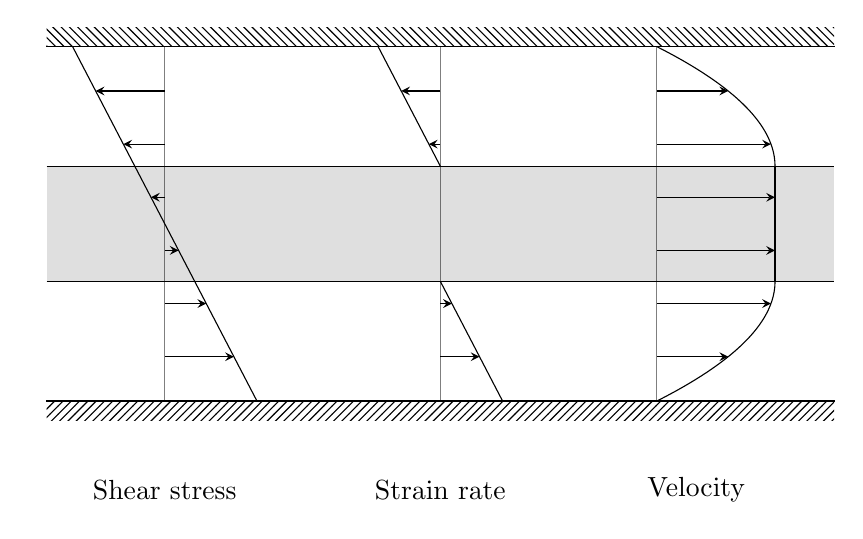
\begin{tikzpicture}
  \tikzstyle{ground1}=[fill,pattern=north west lines,draw=none, minimum width=0.75cm,minimum height=0.2cm]
  \tikzstyle{ground2}=[fill,pattern=north east lines,draw=none, minimum width=0.75cm,minimum height=0.2cm]

  \pgfmathsetmacro{\h}{2.25}
  \pgfmathsetmacro{\l}{5.0}
  \pgfmathsetmacro{\b}{1.3}
  \pgfmathsetmacro{\u}{1.5/(1.-\b/4.)^2}
  \pgfmathsetmacro{\xa}{2.75}
  \pgfmathsetmacro{\xb}{-3.5}
  \pgfmathsetmacro{\xc}{0.0}

  \node (wall_up) [ground1, minimum width=2*\l cm, yshift=\h cm, anchor=south] {};
  \draw (wall_up.south east) -- (wall_up.south west);

  \node (wall_down) [ground2, minimum width=2*\l cm, yshift=-\h cm, anchor=north] {};
  \draw (wall_down.north east) -- (wall_down.north west);

  \fill [gray, opacity=0.25] (-\l,-\b*\h/4) rectangle (\l,\b*\h/4);

  \draw (-\l,\b*\h/4) node[black,anchor=east]{} -- (\l,\b*\h/4) ;
  \draw (-\l,-\b*\h/4) node[black,anchor=east]{} -- (\l,-\b*\h/4) ;
  

  % Stress profile (scaled by 0.4)
  \draw ({\xb+0.4*2.0*(\u)/\h}, -\h) -- ({\xb-0.4*2.0*(\u)/\h}, \h);
  \draw[opacity=0.5] (\xb, -\h) -- (\xb, \h);
  \foreach \eta in {-0.75,-0.45,-0.15,0.15,0.45,0.75} {
    \draw[-stealth] (\xb, \h*\eta) -- ({\xb-0.4*2.0*(\u)/\h*\eta}, \h*\eta);
  }
  \node at (\xb, -1.5*\h) {Shear stress};
  \pause

  % Strain profile
  \foreach \eta in {-0.75,-0.45} {
    \draw[-stealth] (\xc, \h*\eta) -- ({\xc+0.4*(\u)/\h*(-\b/2-2*\eta)}, \h*\eta);
  }
  \foreach \eta in {0.45,0.75} {
    \draw[-stealth] (\xc, \h*\eta) -- ({\xc+0.4*(\u)/\h*(\b/2-2*\eta)}, \h*\eta);
  }
  \draw ({\xc+0.4*(\u)/\h*(-\b/2+2)}, -\h) -- (\xc, -\b*\h/4);
  \draw (\xc, +\b*\h/4) -- ({\xc+0.4*(\u)/\h*(\b/2-2)}, +\h);
  \draw[opacity=0.5] (\xc, -\h) -- (\xc, \h);
  % \draw[-stealth] (\xc, \h*0.75) -- ({\xc-0.75*0.75}, \h*0.75);
  % \draw[-stealth] (\xc, \h*0.45) -- ({\xc-0.45}, \h*0.45);
  % %\draw[-stealth] (\xc, \h*0.15) -- ({\xc}, \h*0.15);
  % % \draw[-stealth] (\xc, -\h*0.15) -- ({\xc+0.15}, -\h*0.15);
  % \draw[-stealth] (\xc, -\h*0.45) -- ({\xc+0.45}, -\h*0.45);
  % \draw[-stealth] (\xc, -\h*0.75) -- ({\xc+0.75}, -\h*0.75);
  \node at (\xc, -1.5*\h) {Strain rate};
  \pause

  % Velocity profile
  \draw[opacity=0.5] (\xa+0, -\h) -- (\xa+0, \h);
  \draw ({\xa+\u*(1-\b/4)^2}, -\b*\h/4) -- ({\xa+\u*(1-\b/4)^2}, \b*\h/4);
  \draw  plot[smooth,domain={\b/4}:1] ({\u*((1-\x^2)-\b/2*(1-\x))+\xa}, {\h * \x});
  \draw  plot[smooth,domain={\b/4}:1] ({\u*((1-\x^2)-\b/2*(1-\x))+\xa}, {-\h*\x});
  \draw[-stealth] (\xa, \h*0.75) -- ({\u*((1-(0.75)^2)-\b/2*(1-0.75))+\xa}, \h*0.75);
  \draw[-stealth] (\xa, \h*0.45) -- ({\u*((1-(0.45)^2)-\b/2*(1-0.45))+\xa}, \h*0.45);
  \draw[-stealth] (\xa, \h*0.15) -- ({\xa+\u*(1-\b/4)^2}, \h*0.15);
  \draw[-stealth] (\xa, -\h*0.15) -- ({\xa+\u*(1-\b/4)^2}, -\h*0.15);
  \draw[-stealth] (\xa, -\h*0.45) -- ({\u*((1-(0.45)^2)-\b/2*(1-0.45))+\xa}, -\h*0.45);
  \draw[-stealth] (\xa, -\h*0.75) -- ({\u*((1-(0.75)^2)-\b/2*(1-0.75))+\xa}, -\h*0.75);
  \node at ({\xa+0.5}, -1.5*\h) {Velocity};
  
  \onslide<1->
\end{tikzpicture}

    \end{figure}
\end{frame}

\begin{frame}{Interface tracking benefits - Poiseuille flow}
    \begin{figure}
        %\centering
        \begin{overprint}
            \onslide<1>\includesvg[width=\textwidth]{../figures/res_P1_first.svg}
            \onslide<2>\includesvg[width=\textwidth]{../figures/res_P1_last.svg}
            \end{overprint} 
    \end{figure}
\end{frame}

%---------------------------------------------------------

\section{How do we model it ?}
\subsection{Differential equations}

\begin{frame}{Equations}
    \begin{itemize}
        %\setlength{\itemsep}{-6pt}
        \item Conservation laws for incompressible fluids\only<2>{, with low Reynolds}:
        \begin{align*}
            \nabla \cdot \vv &= 0 & \text{in } \Omega\\
            \only<1>{\rho \left(\pdv{\vv}{t} + \left(\vv \cdot \nabla\right) \vv\right) &= -\nabla p + \nabla \cdot \boldsymbol\tau + \mathbf{f}}
            \only<2->{0 &= -\nabla p + \nabla \cdot \boldsymbol\tau + \mathbf{f}}
            & \text{in } \Omega
        \end{align*}
        \pause[3]
        \item Constitutive law
        \begin{align*}
            \boldsymbol{\dot\gamma} &= 0 & \text{if} \quad \tau < \tau_0\\
            \boldsymbol\tau &= \left(K + \tau_0/\dot\gamma\right) \boldsymbol{\dot\gamma} & \text{if} \quad \tau \geq \tau_0
        \end{align*}
        \pause
        \item Boundary conditions
        \begin{align*}
            \vv &= \mathbf{U} & \text{on } \partial \Omega_{D}\\
            \mathbf{\hat n} \cdot \boldsymbol\sigma &= \mathbf{g} & \text{on } \partial \Omega_{N}
        \end{align*}
    \end{itemize}
\end{frame}

\begin{frame}{Energy functional}
    System of PDE's is equivalent to
    \begin{align*}
        \vv &= \argmin_{\uu \in \mathcal{V}} \mathcal{J}(\uu)\\[8pt]
        \mathcal{V} &= \left\{\uu \in H^1(\Omega)^d \;\Big\vert\; \int_{\Omega}q \nabla \cdot \uu \; \dd x = 0 \;\; \forall q \in L^2(\Omega), \: \uu = \mathbf{U} \;\text{on}\; \partial \Omega_D \right\}\\[8pt]
        \mathcal{J}(\uu) &= \overbrace{\frac{K}{2}\int_{\Omega} \|\gam(\uu)\|^2 \;\dd x}^{\text{Viscous}} + \overbrace{\tau_0 \int_{\Omega} \|\gam(\uu)\| \;\dd x}^{\text{Yield}} 
         - \underbrace{\int_{\Omega} \ff\cdot \uu \; \dd x}_{\text{Body forces}} - \underbrace{\int_{\partial \Omega_N} \mathbf{g} \cdot \uu \;\dd s}_{\text{Boundary forces}}
    \end{align*}
\end{frame}

\subsection{Finite elements}
\begin{frame}{Finite element method: a stable discretization ?}
    Discretize velocity-pressure fields, over a mesh of triangles, with either:
    \begin{itemize}
        \item Mini element: $(\mathcal{P}_1^C\oplus \mathcal{B}_3^C) - \mathcal{P}_1^C$
        \item Taylor-Hood element: $\mathcal{P}_2^C - \mathcal{P}_1^C$
    \end{itemize}
    \begin{figure}
        \begin{overprint}
            \onslide<2>
            \centering
            \includesvg[width=0.75\textwidth]{../figures/shape_fcts_2d_P1.svg}
            %\caption{$\mathcal{P}_1$}
            \onslide<3>
            \centering
            \includesvg[width=0.75\textwidth]{../figures/shape_fcts_2d_bubble.svg}
            %\caption{$\mathcal{P}_1 \oplus \mathcal{B}_3$}
            \onslide<4>
            \centering
            \includesvg[width=0.90\textwidth]{../figures/shape_fcts_2d_P2.svg}
            %\caption*{$\mathcal{P}_2$}
        \end{overprint}
    \end{figure}
\end{frame}


\begin{frame}{Finite element approximation}
    \begin{itemize}
    \item Finite element approximation:
    \begin{equation*}
        \vv^h(\xx) = \sum_{\text{nodes } j} \mathbf{V}_{j} \phi_j(\xx)
    \end{equation*}
    \item Discrete functional\only<2>{, with additional variables $S_{i,g}$ and $T_{i,g}$}:
    \begin{align*}
        \mathcal{J}(\vv^h) &= \sum_{i}\sum_{g} \omega_g \left[\frac{K}{2} 
        \onslide<2-> \overbrace{
            \onslide<1-> \|\gam(\vv^h)\|^2 \onslide<2->
        }^{\leq S_{i,g}} \onslide<1->
        + \tau_0 
        \onslide<2-> \overbrace{
            \onslide<1-> \color{red!70} \|\gam(\vv^h)\| \color{black} \onslide<2->
        }^{\leq T_{i,g}} \onslide<1->
        - \mathbf{f} \cdot \vv^h \right] \det \dv{\mathbf{x}}{\boldsymbol \xi}_{i,g}\\
        &\quad -\sum_{e}\sum_{g} \tilde \omega_g \,\mathbf{g}\cdot \vv^h \;\det \dv{\mathbf{\tilde x}}{\boldsymbol \tilde \xi}_{e,g}
    \end{align*}
    \end{itemize}
\end{frame}

\subsection{Conic optimization}
\begin{frame}{Objective and constraints}
    \small
    \begin{alignat*}{2}
        \minimize_{\mathbf{V}_j, S_{i,g}, T_{i,g}} \quad &\sum_{i,g} \omega_g \left[\frac{K}{2} S_{i,g} + \tau_0 T_{i,g} - \mathbf{f} \cdot \vv^h \right] \det \dv{\mathbf{x}}{\boldsymbol \xi}_{i,g} - \sum_{e,g} \tilde \omega_g \,\mathbf{g}\cdot \vv^h &&\det \dv{\mathbf{\tilde x}}{\boldsymbol \tilde \xi}_{e,g}\\[8pt]
        \text{such that} \quad & S_{i,g} \geq (2\partial_x{u^h})^2 + (2\partial_y{v^h})^2 + (\partial_y{u^h}+\partial_x{v^h})^2 && \forall i, g\\
        &T_{i,g} \geq \sqrt{(2\partial_x{u^h})^2 + (2\partial_y{v^h})^2 + (\partial_y{u^h}+\partial_x{v^h})^2} && \forall i, g\\
        &0 = \sum_{i,g} \omega_g q_l \vert_{\xx_g} \left(\partial_x u^h + \partial_y v^h\right) \det \dv{\mathbf{x}}{\boldsymbol \xi}_{i,g} && \forall\; l\\
        &\mathbf{V}_{j} = \mathbf{U} && \forall\; j \in \partial\Omega_D
    \end{alignat*}
    \normalsize
\end{frame}

\begin{frame}{Reformulation for conic optimization}
    \small
    \begin{alignat*}{2}
        \minimize_{\mathbf{V}_j, S_{i,g}, T_{i,g}} \quad &\sum_{i,g} \omega_g \left[\frac{K}{2} S_{i,g} + \tau_0 T_{i,g} - \mathbf{f} \cdot \vv^h \right] \det \dv{\mathbf{x}}{\boldsymbol \xi}_{i,g}-\sum_{e,g} \tilde \omega_g \,\mathbf{g}\cdot \vv^h &&\det \dv{\mathbf{x}}{\boldsymbol \xi}_{e,g}\\[8pt]
        \text{such that} \quad & 0 \preceq_{L^5_R} \left(S_{i,g}, \frac{1}{2}, \sqrt{2}\partial_x u^h, \sqrt{2}\partial_y v^h, \partial_y u^h+\partial_x v^h\right) && \forall i, g\\
        & 0 \preceq_{L^4} \left(T_{i,g}, \sqrt{2}\partial_x u^h, \sqrt{2}\partial_y v^h, \partial_y u^h+\partial_x v^h\right) && \forall i, g\\
        &0 = \sum_{i,g} \omega_g q_l \vert_{\xx_g} \left(\partial_x u^h + \partial_y v^h\right) \det \dv{\mathbf{x}}{\boldsymbol \xi}_{i,g} && \forall\; l\\
        &\mathbf{V}_{j} = \mathbf{U} && \forall\; j \in \partial\Omega_D
    \end{alignat*}
    \normalsize
    \pause
    \vspace{-12pt}
    \begin{itemize}
        \item Objective is linear in variables $U_j$, $V_j$, $S_{i,g}$, $T_{i,g}$
        \item Equality constraints are linear
        \item Inequality constraints are proper cones
    \end{itemize}
\end{frame}

\begin{frame}{Conic solver}
    Can find the optimum with an interior-point method:
    \begin{itemize}
        \item Encode each constraint with barrier $g_n$
        \item Minimize a modified functional $\mathcal{J} + \mu\sum g_n$
        \item Alternatively:
        \begin{itemize}
            \item Perform Newton iterations (stay optimal)
            \item Decrease $\mu \to 0$ (minimize original objective $\mathcal{J}$)
        \end{itemize} 
        \item Proper cones provide special barriers (self-concordant)
        \item Solution obtained with Newton–Raphson method, within accuracy $\epsilon$, after $\mathcal{O}(\sqrt{\nu} \log \frac{1}{\epsilon})$ iterations, where $\nu\propto$ number of variables
    \end{itemize}
\end{frame}

\begin{frame}{Interior-point solver example}
    \begin{figure}
        \centering
        %\movie[width=0.7\textheight, height=0.7\textheight, showcontrols]{} {../anim/interior_point.mp4}
        \animategraphics[autoplay,loop,width=0.5\textwidth]{15}{../anim/interior_point/frame}{1}{76}
        \caption*{Minimize $x$ with linear inequalities over $x$ and $y$}
    \end{figure}
\end{frame}

\subsection{Interface tracking}
\begin{frame}{Interface tracking}
    Once we have the velocity field, minimum of $\mathcal{J}$:
    \begin{enumerate}
        %\item Find the velocity field $\vv$ by minimizing $\mathcal{J}$
        \item Estimate the interface position based on the strain rate field $\gam(\vv^h)$
        \begin{itemize}
            \item Not trivial, as it is not a level set of $\dot\gamma$
        \end{itemize}
        \item Move the nodes of the mesh towards the interface estimation
        \begin{itemize}
            \item X-MESH algorithm allowing extreme deformations of the mesh
        \end{itemize}
    \end{enumerate}
    
    % $\dot\gamma=0$ everywhere inside the rigid regions
    % $C^2$ discontinuity at the interface
    % The interface is \textbf{not} a level-set of a scalar field.
\end{frame}

\begin{frame}{Locating the interface}
    \begin{figure}
        \centering
        \begin{tikzpicture}
            \draw[-Latex] (-4., 0.) -- (-4., 4.) node[right] {$\dot \gamma$};
            \draw[-Latex] (-4., 0.) -- (4., 0.) node[above] {$x$};
            \draw[line width=1mm] (-4., 0.) -- (-1., 0.) node[pos=0.4, above] {\small Rigid region};
            \draw[line width=1mm] ({sqrt(2)/2.}, {sqrt(2)/2.}) -- (4., 4.);
            \node[above] at (2.5, 0.) {\small Liquid region};
            % \draw[dashed] (0., -0.5) -- (0., 1.) node[pos=0., below] {Interface};
            \draw (0., 0.) circle[radius=1 cm];
            \only<1>{\node[align=center] {\small Interface not \\ \small well resolved};}
            \only<2->{\draw[red] (1., 1.05) node {\Large$\boldsymbol\times$};}
            \only<2->{\draw[red] (2., 2.15) node {\Large$\boldsymbol\times$};}
            \only<2->{\draw[red] (3., 3.15) node {\Large$\boldsymbol\times$};}
            \only<3->{\draw[red, dashed, thick] (-1., -1.) -- (3., 3.15) node[pos=0.55,above=6pt] {$\phi$};}
            \only<4>{\fill[red] (-0.01, 0.) circle[radius=4pt] node[below] {\small Estimation};}
        \end{tikzpicture}
        %\caption*{Scalar strain rate $\dot\gamma$ near an interface}
    \end{figure}
\end{frame}

\begin{frame}{Locating the interface - Predictor}
    \begin{figure}
        \centering
        \includesvg[width=0.5\textwidth]{../figures/rec_2.svg}
    \end{figure}
\end{frame}

\begin{frame}{Locating the interface - Compute linear approximation}
    \begin{figure}
        \centering
        \includesvg[width=0.5\textwidth]{../figures/rec_3.svg}
    \end{figure}
\end{frame}

\begin{frame}{Locating the interface - Evaluate linear approximation}
    \begin{figure}
        \centering
        \includesvg[width=0.5\textwidth]{../figures/rec_4.svg}
    \end{figure}
\end{frame}

\begin{frame}{Locating the interface - Average linear approximations}
    \begin{figure}
        \centering
        \includesvg[width=0.5\textwidth]{../figures/rec_7.svg}
    \end{figure}
\end{frame}

% \begin{frame}{In practice}
%     \begin{figure}
%         \begin{overprint}
%             \only<1>{\centering\includesvg[width=0.9\textwidth]{../figures/rect_init.svg}}
%             \only<2>{\centering\includesvg[width=0.9\textwidth]{../figures/rect_last.svg}}
%         \end{overprint}
%     \end{figure}
% \end{frame}

%---------------------------------------------------------

\section{Numerical results}

\begin{frame}{Curved channel}
    \begin{figure}
        \centering
        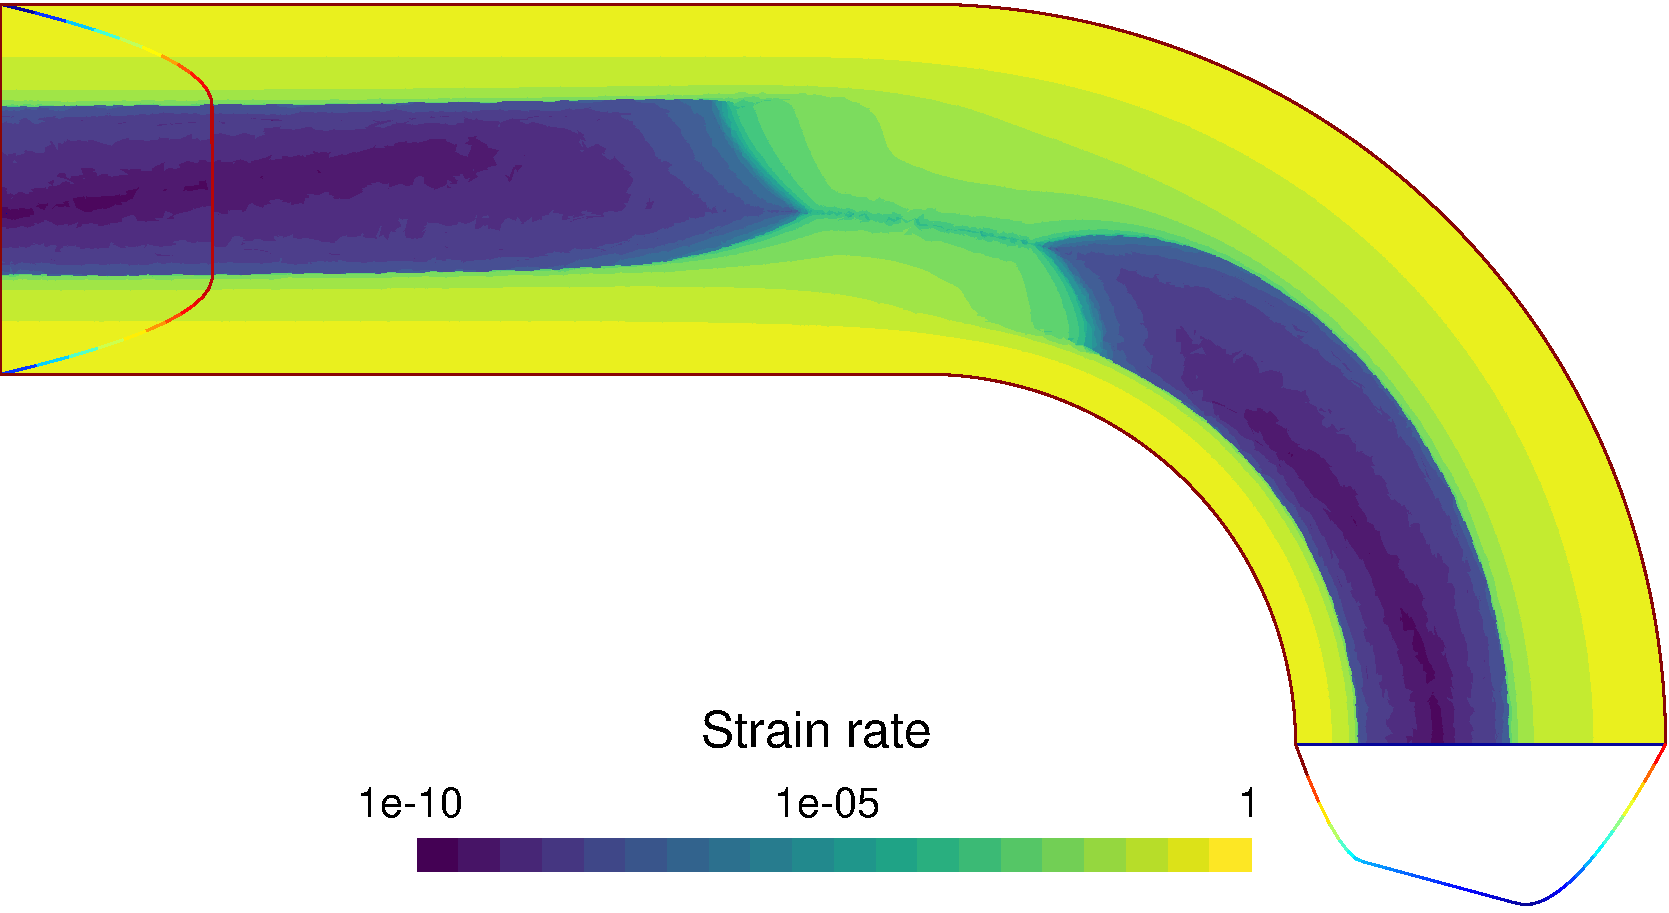
\includegraphics[width=0.9\textwidth]{../figures/pipe_strain_v2.pdf}
    \end{figure}
\end{frame}

\begin{frame}{Curved channel - Pressure discontinuity}
    Jump condition 
    \begin{equation*}
        \llbracket\boldsymbol\sigma\cdot \nn \rrbracket = 0 \implies \llbracket p \nn \rrbracket = \llbracket\boldsymbol\tau\cdot \nn \rrbracket = {\color{gray!50} \llbracket K \gam \cdot \nn \rrbracket} + \tau_0 \llbracket \gam/\dot\gamma \cdot \nn \rrbracket
    \end{equation*}
    \begin{figure}
        \begin{overprint}
            \only<1>{\centering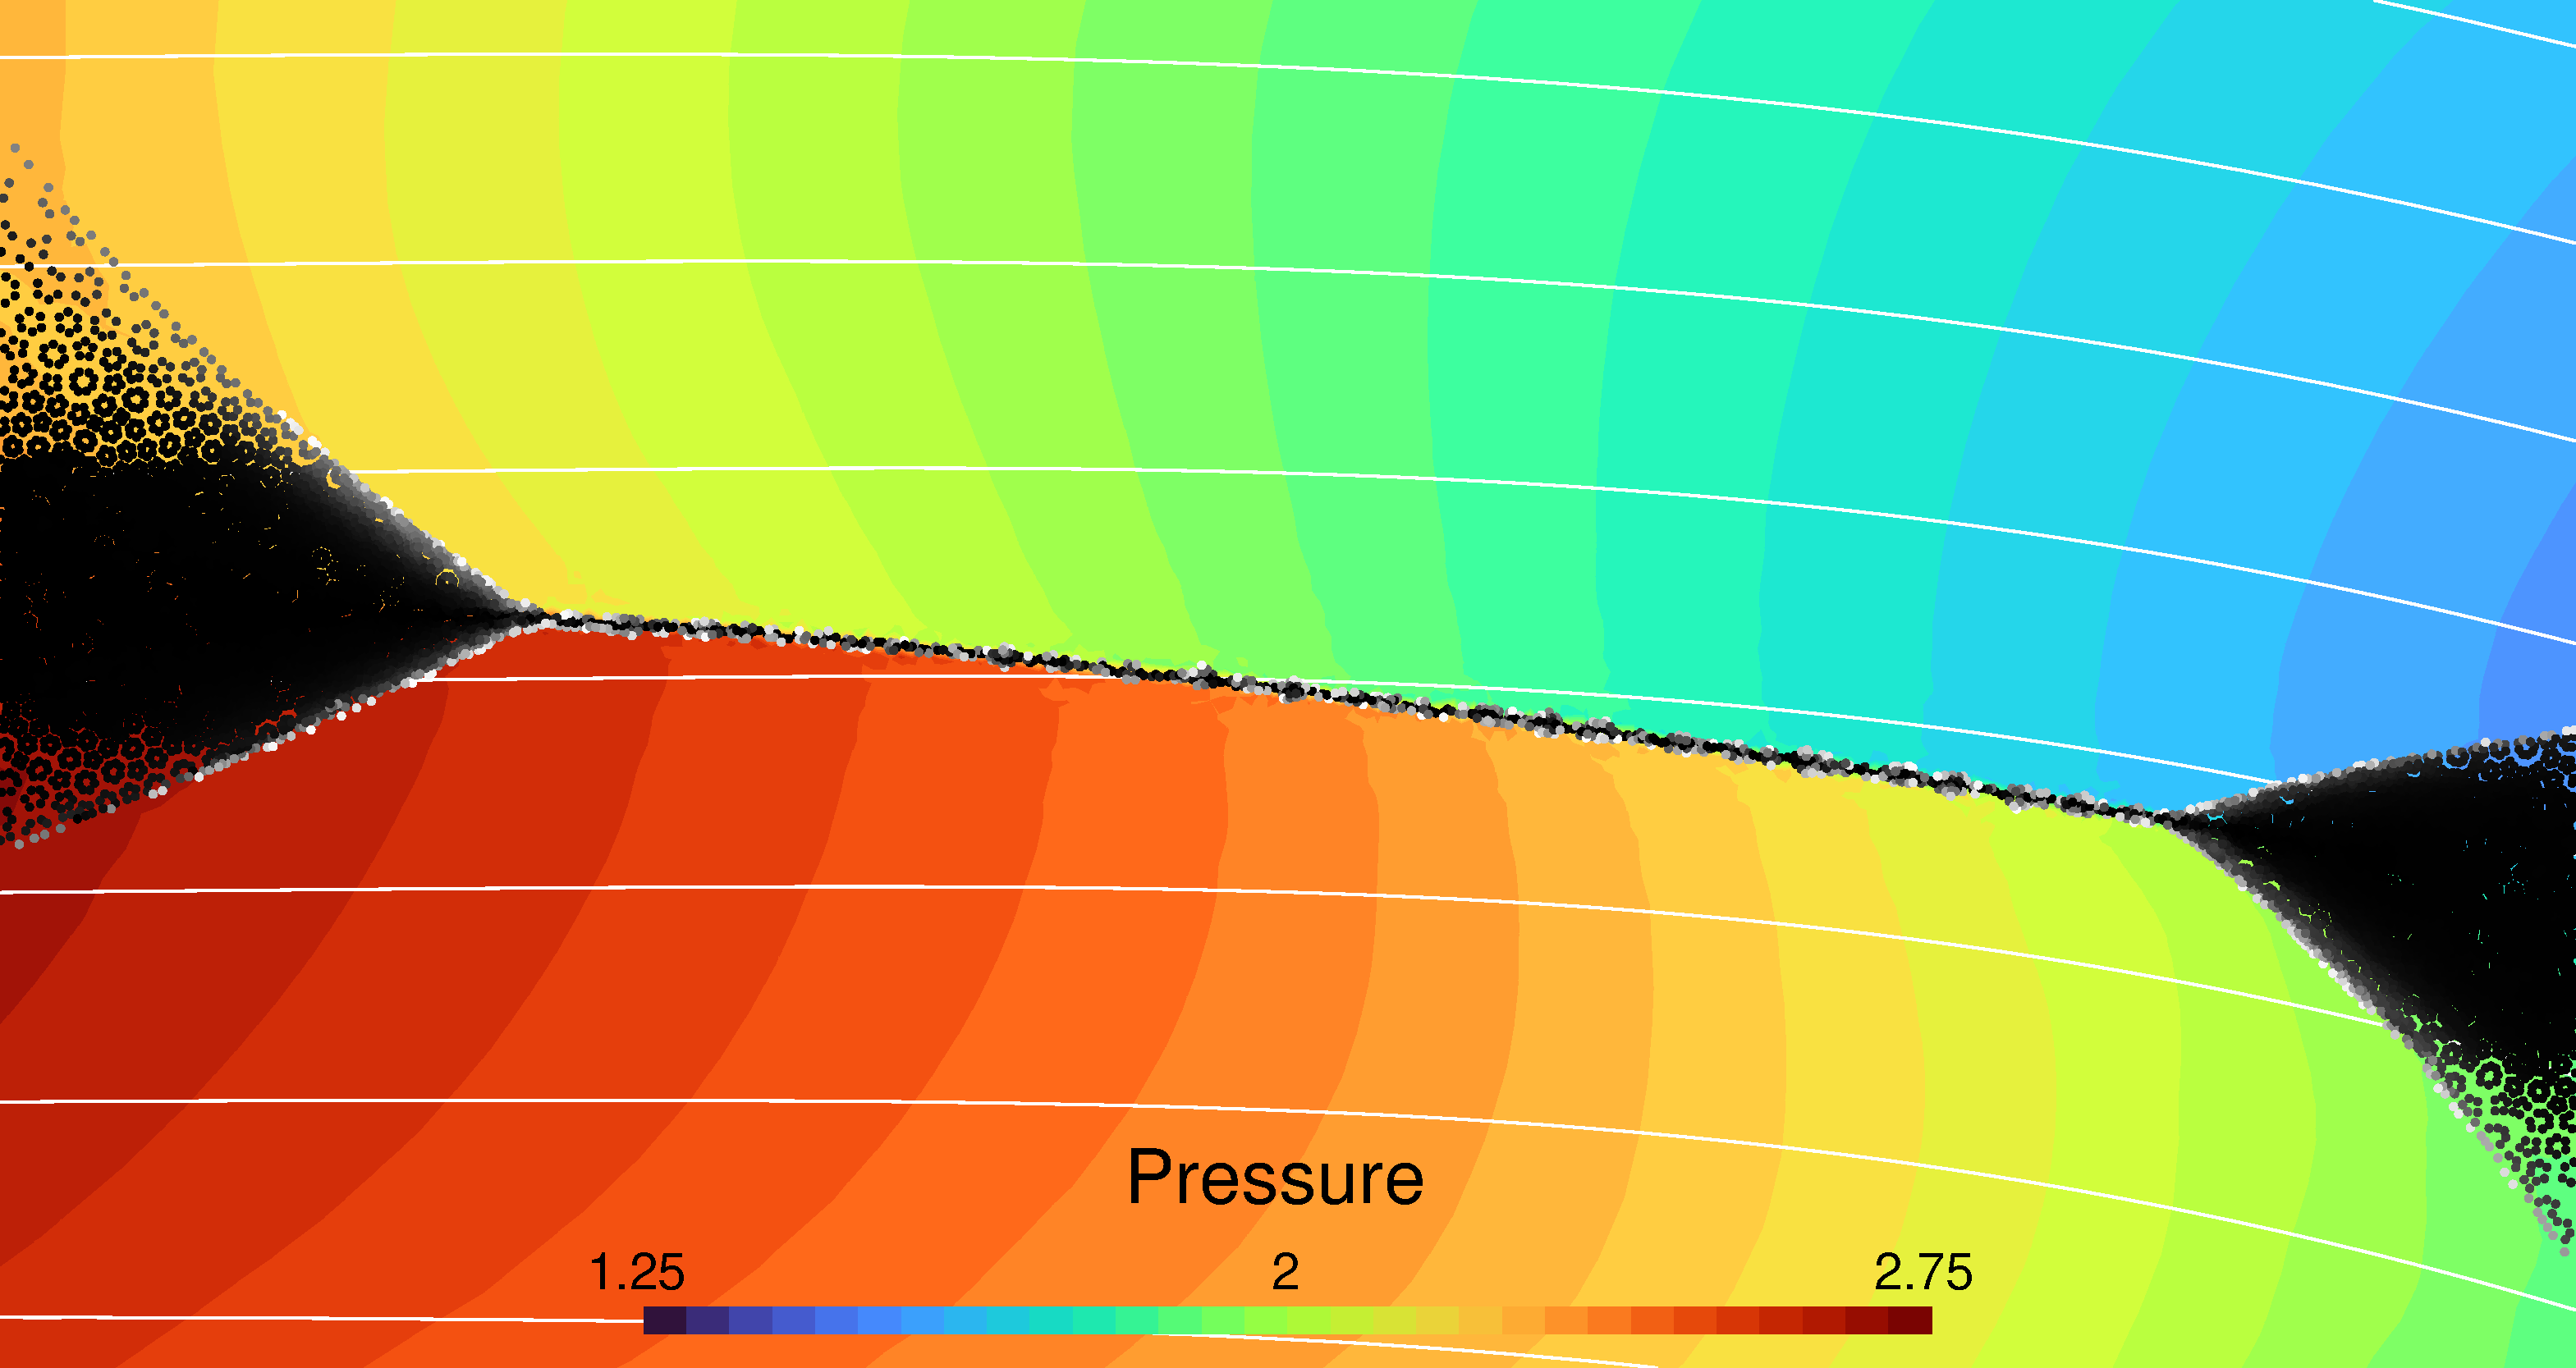
\includegraphics[width=0.85\textwidth]{../figures/pipe_filament_p.pdf}}
            \only<2>{\centering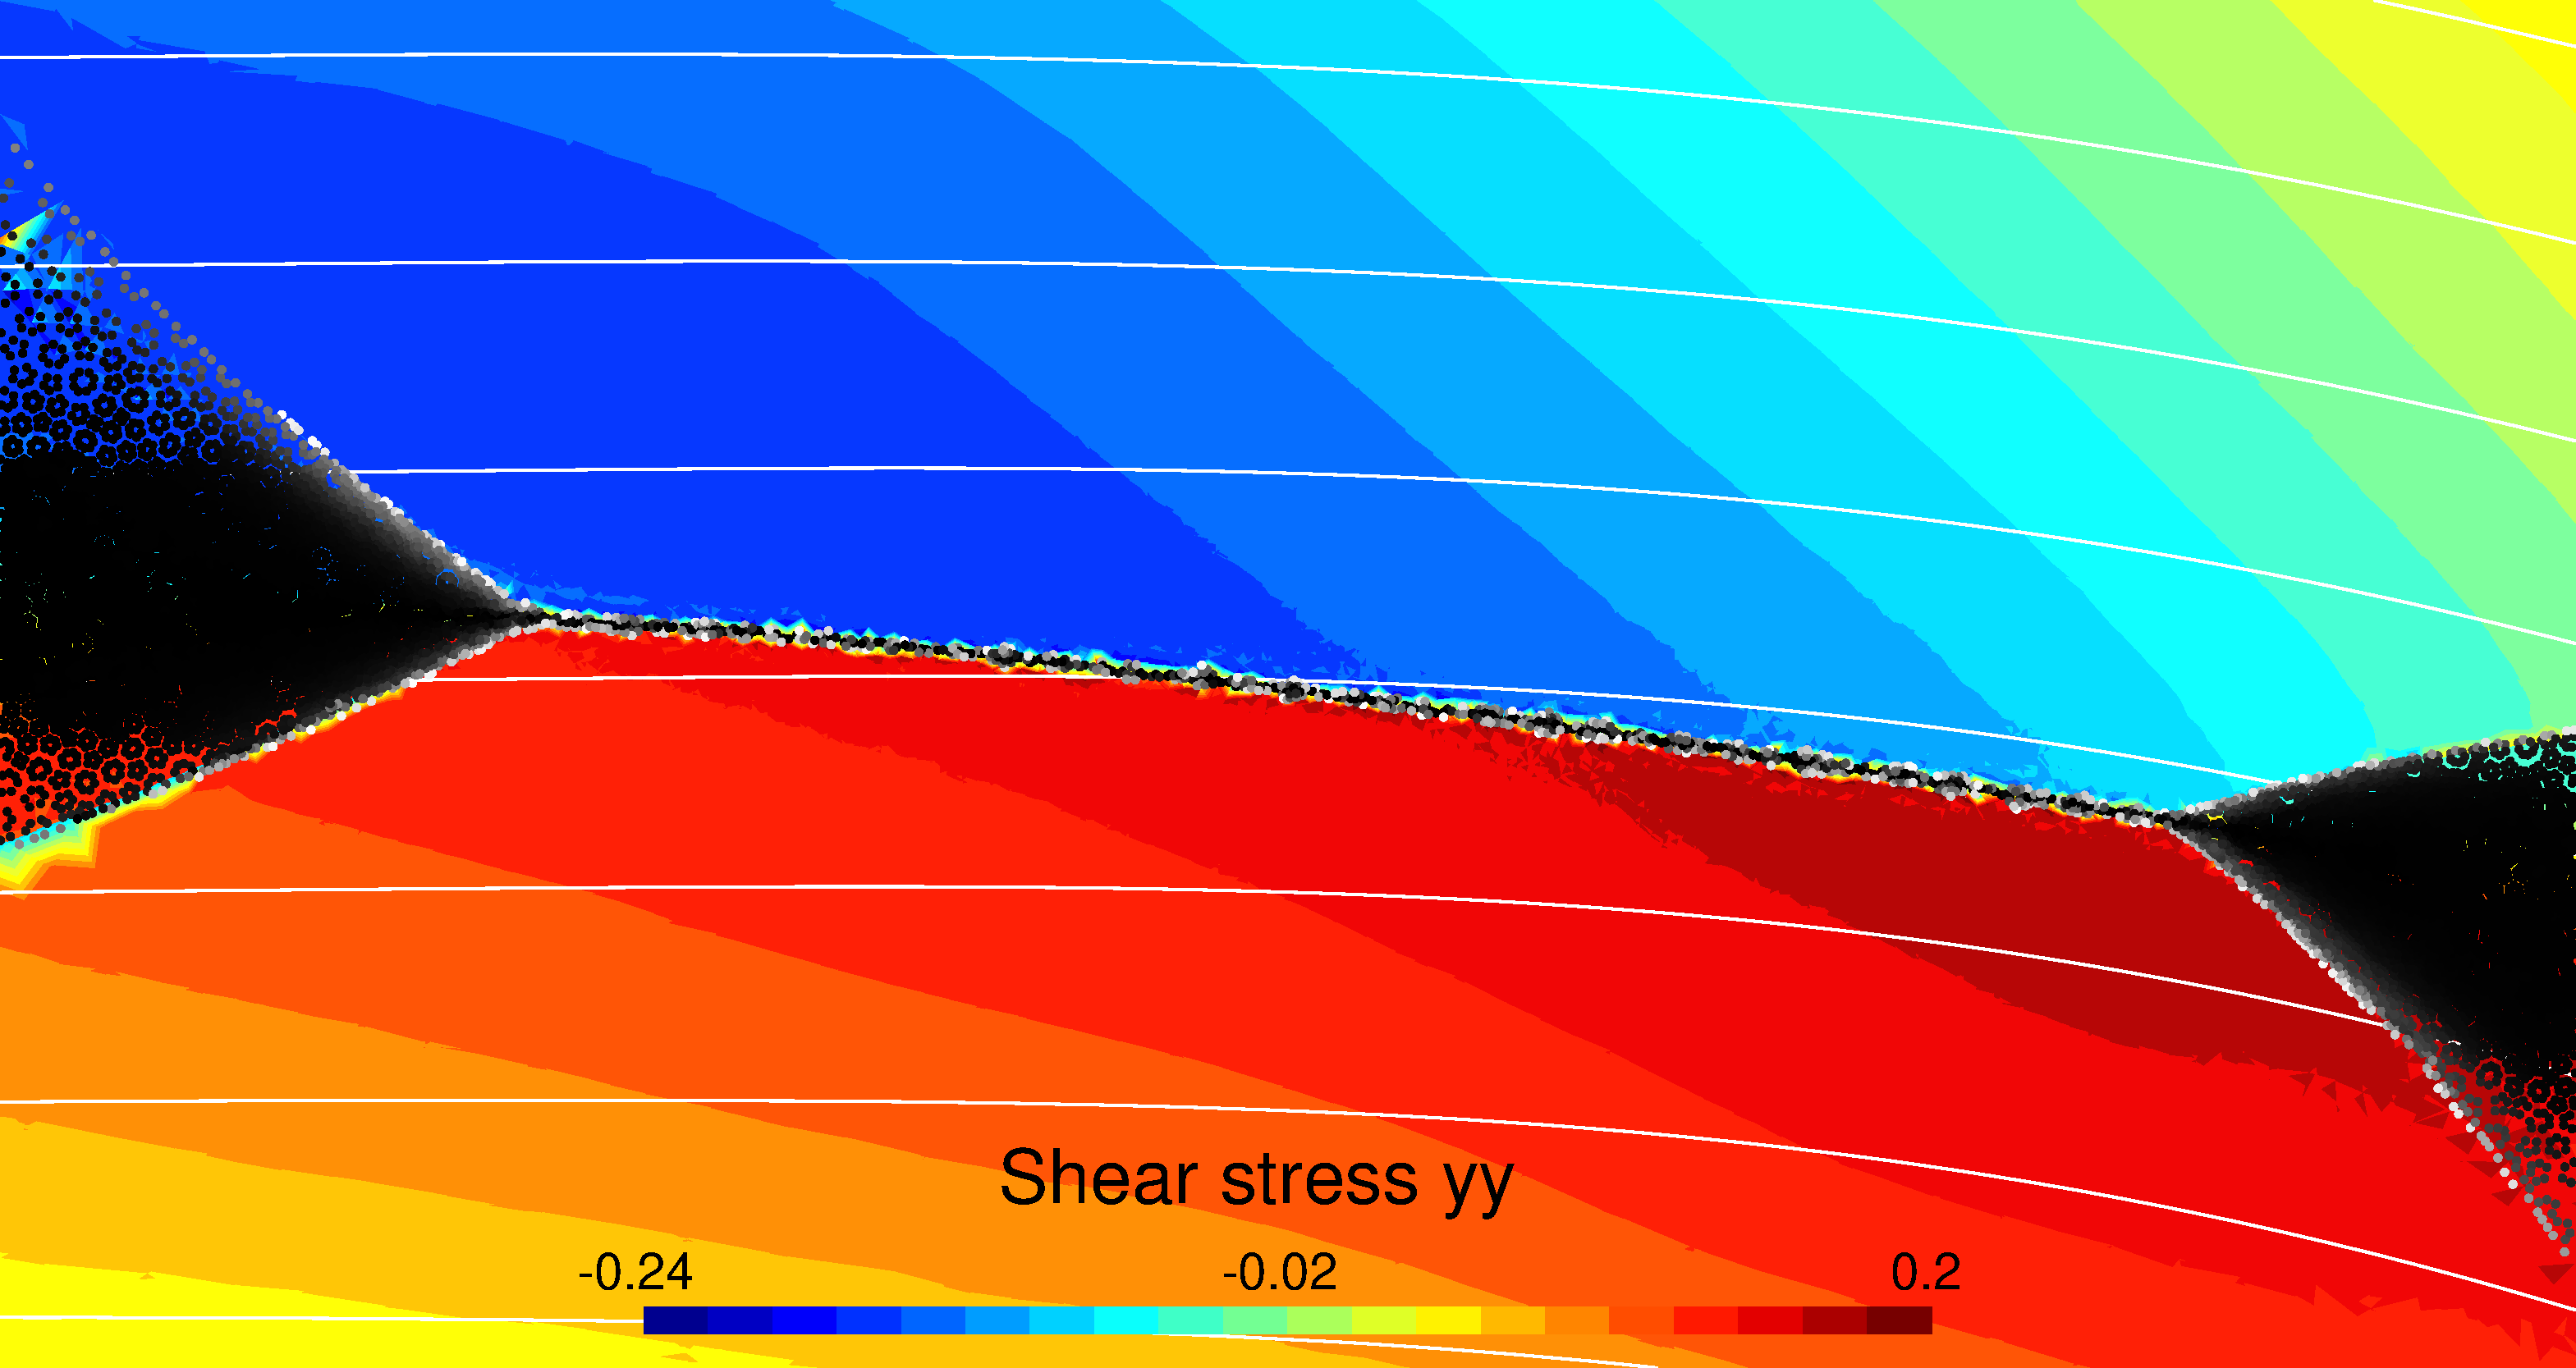
\includegraphics[width=0.85\textwidth]{../figures/pipe_filament_d.pdf}}
        \end{overprint}
    \end{figure}
\end{frame}

\begin{frame}{Curved channel - Increasing Bingham}
    \begin{figure}
        %\movie[width=0.8\textwidth, height=0.52\textwidth, showcontrols]{} {../anim/filament.mp4}
        \animategraphics[autoplay,loop,width=0.8\textwidth]{4}{../anim/filament_focus/frame}{1}{21}
    \end{figure}
\end{frame}

\begin{frame}{Lid-driven cavity}
    \begin{figure}[htb]
        \centering
        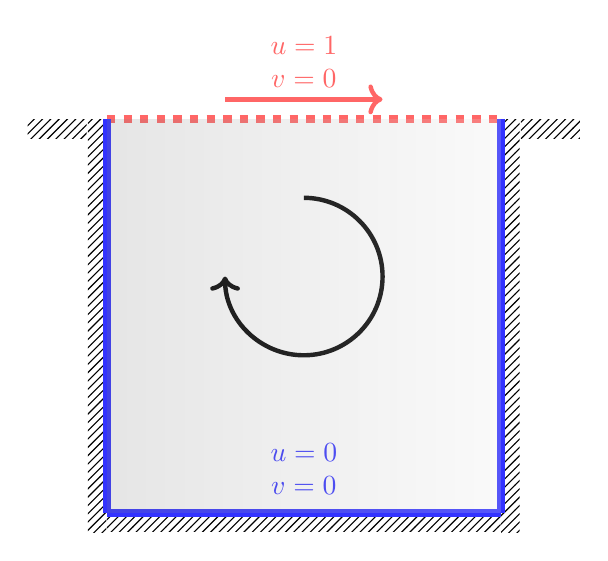
\begin{tikzpicture}
            \pgfmathsetmacro{\x}{0.}
            \pgfmathsetmacro{\l}{2.5}
            \tikzstyle{groundDw}=[fill,pattern=north east lines,draw=none, minimum width=0.75cm,minimum height=0.2cm]
            \tikzstyle{groundLf}=[fill,pattern=north east lines,draw=none, minimum width=0.2cm,minimum height=0.75cm]
            
            %%%%%%%%%%%%%%%%%%%%%%%%%%%%%%%%%%%%%%%%
            \draw[dashed, line width=1mm, red!60] (-\x-\l,\l) -- (-\x+\l,\l);
    
            \node at (-\x, 0) (wall_down) [groundDw, minimum width=2*\l cm, yshift=-\l cm,anchor=north] {};
            \draw[line width=1mm, blue!80] (-\x-\l,-\l) -- (-\x+\l,-\l);
            
            \node at (-\x, 0.) (midL) [groundLf, minimum height=2.1*\l cm, xshift=-\l cm, yshift=-0.05*\l cm, anchor=east] {};
            \draw[line width=1mm, blue!80] (-\x-\l,-\l) -- (-\x-\l,+\l);
            
            \node at (-\x, 0.) (midR) [groundLf, minimum height=2.1*\l cm, xshift=+\l cm, yshift=-0.05*\l cm, anchor=west] {};
            \draw[line width=1mm, blue!80] (-\x+\l,-\l) -- (-\x+\l,+\l);
            
            \node at (-\x-\l, \l) (topL) [groundDw, minimum width=0.3*\l cm, xshift=-0.1*\l cm, yshift=-0.05*\l cm, anchor=east] {};
            \node at (-\x+\l, \l) (topR) [groundDw, minimum width=0.3*\l cm, xshift=0.1*\l cm, yshift=-0.05*\l cm, anchor=west] {};
            \node[above=3pt,blue!80,align=center] at (-\x, -\l) {$u=0$\\$v=0$};
            
            \draw[ultra thick, red!60, ->] (-\x-1,\l*1.1) -- (-\x+1,\l*1.1) node[midway, above, red!60,align=center] {$u=1$ \\ $v=0$};
            \draw[ultra thick, ->] (-\x,\l*0.6) arc (90:-180:1);
            
            \node [
                opacity=0.2, shading=axis, rectangle, shading angle=180,
                left color=gray,  right color=gray!20!white,
                minimum width=2*\l cm,  minimum height=2*\l cm
                ] (box) at (-\x, 0.){};
        \end{tikzpicture}
    \end{figure}
\end{frame}

\begin{frame}{Lid-driven cavity - before/after interface tracking}
    \begin{figure}
        \begin{overprint}
            \only<1>{\centering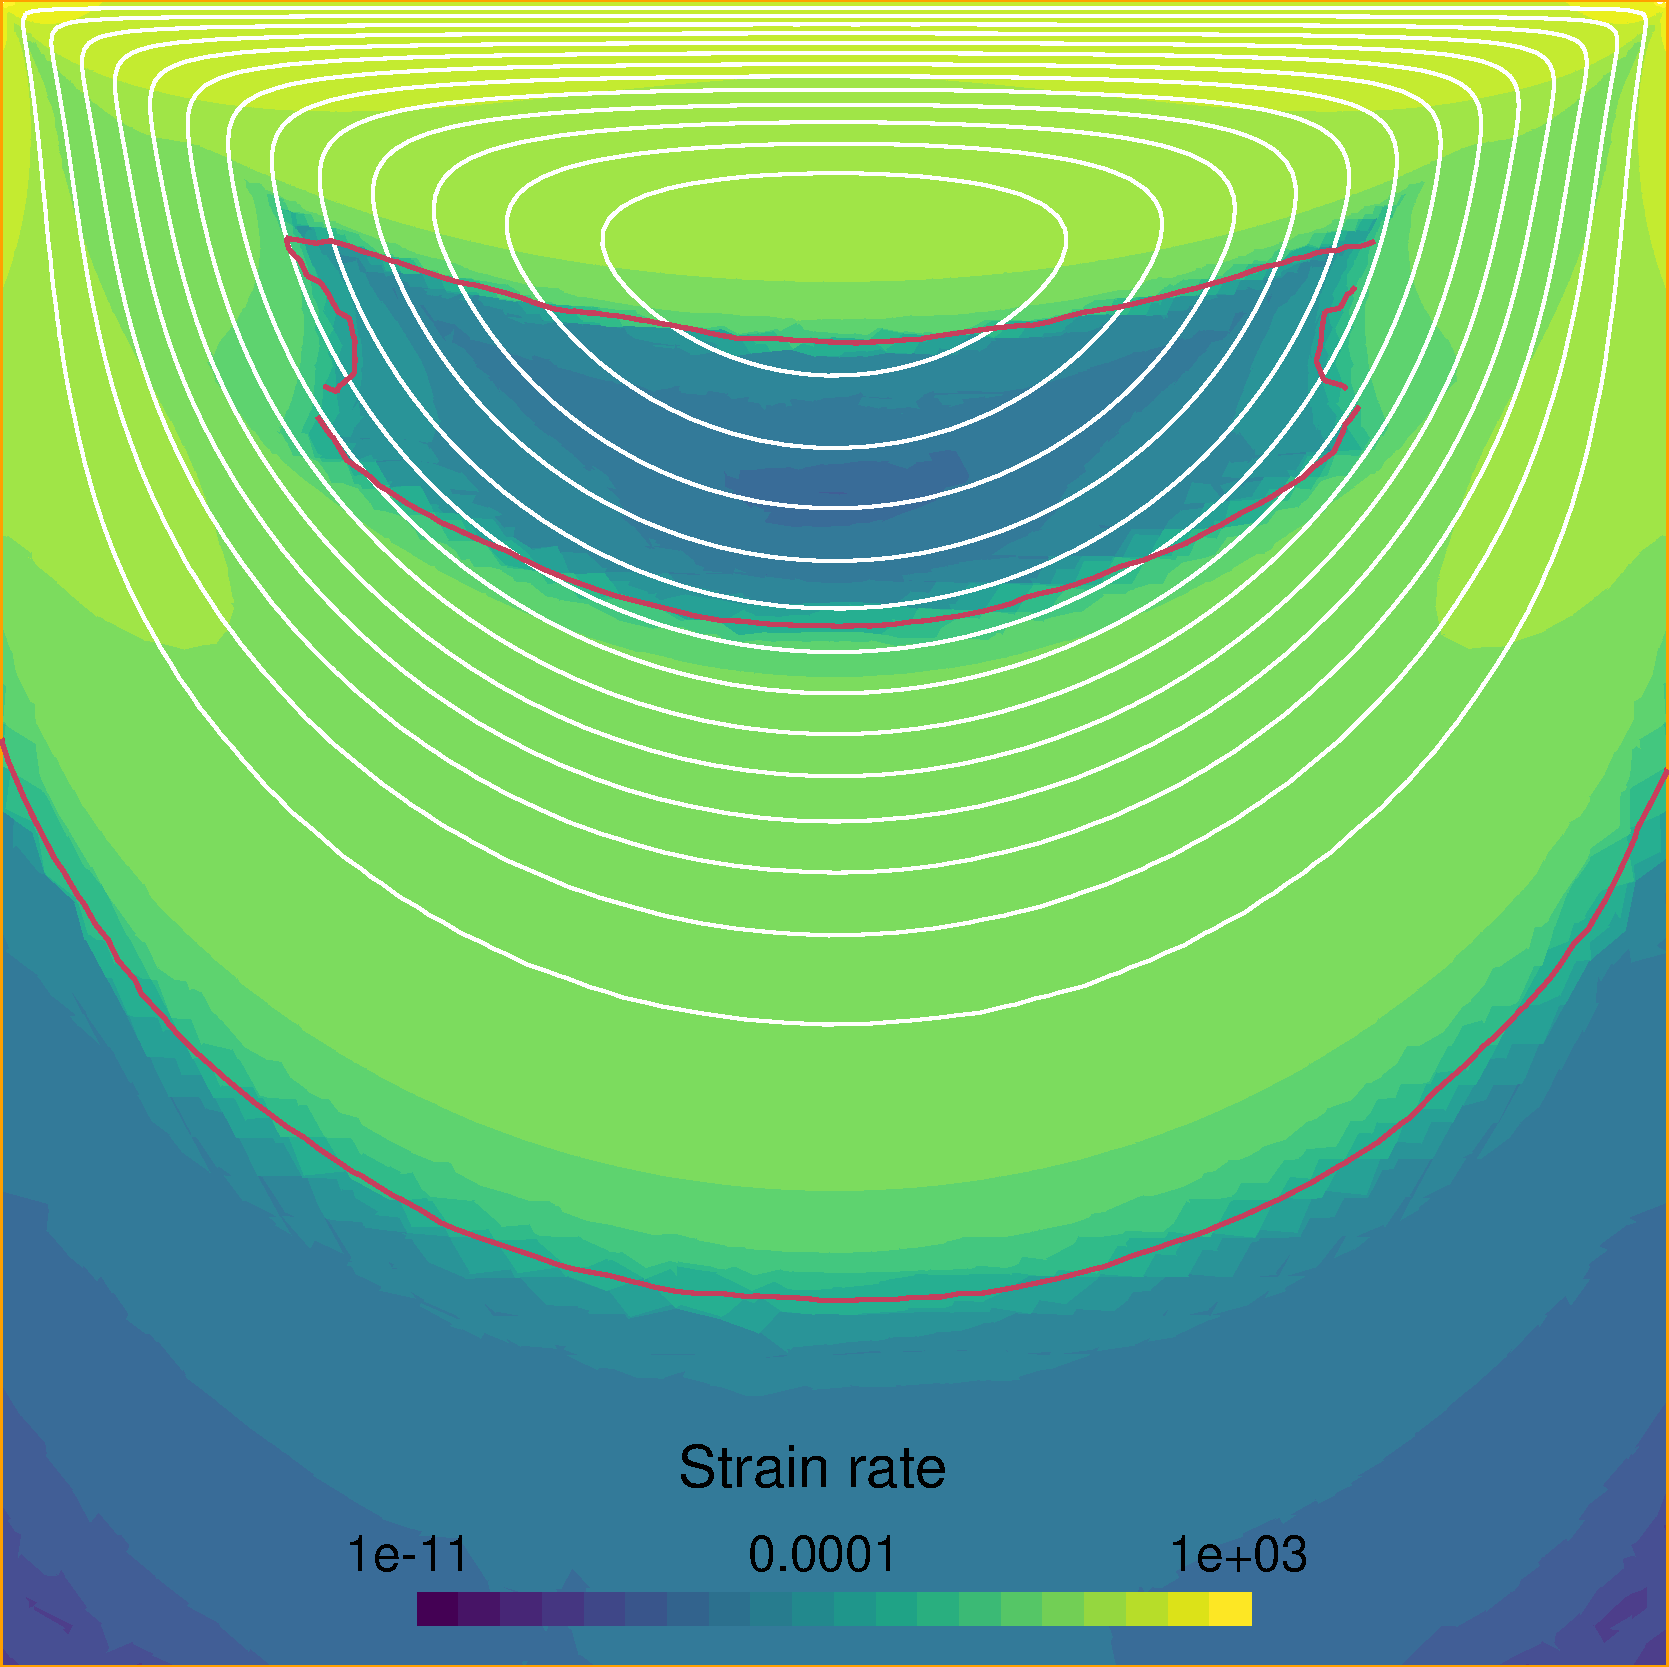
\includegraphics[height=0.75\textheight]{../figures/cavity_init.pdf}}
            \only<2>{\centering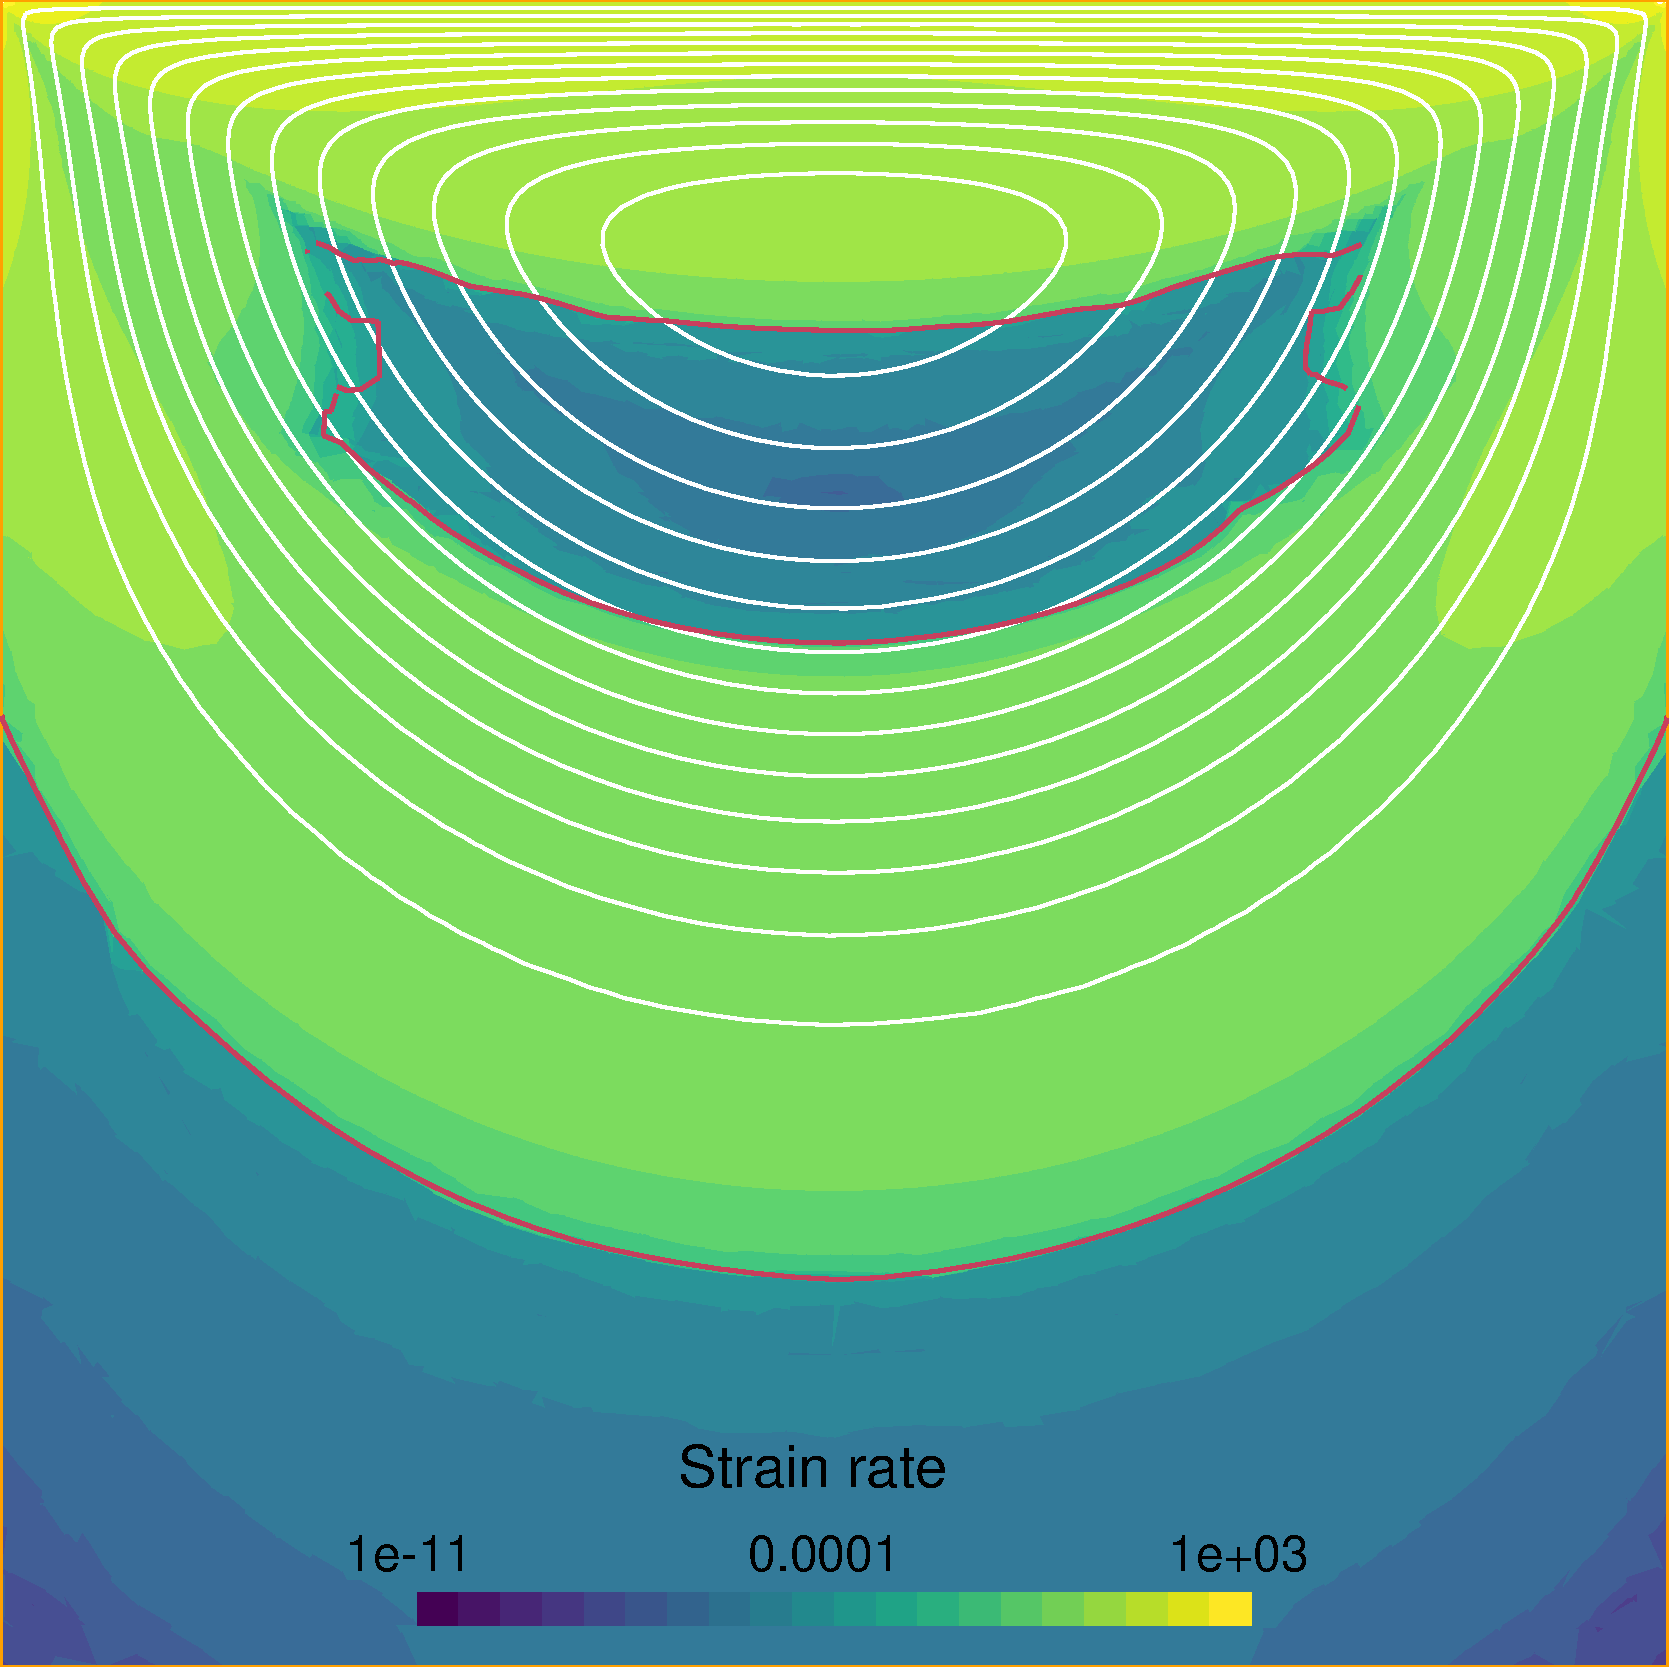
\includegraphics[height=0.75\textheight]{../figures/cavity_last.pdf}}
        \end{overprint}
    \end{figure}
\end{frame}

\begin{frame}{Lid-driven cavity - comparison with the literature}
    \begin{figure}
        \centering
        \includesvg[width=0.80\textwidth]{../figures/profile_papers_cavity.svg}
    \end{figure}
\end{frame}

\begin{frame}{Lid-driven cavity - Rigid body motion}
    \begin{figure}
        \centering
        \begin{subfigure}[t]{0.48\textwidth}
            \movie[width=\textwidth, height=1.042\textwidth, autostart, loop]{} {../anim/cavity_20/cavity_20.mp4}
            % \animategraphics[autoplay,loop,width=\textwidth]{25}{../anim/cavity_20/frame_}{1}{100}
        \end{subfigure}
        \begin{subfigure}[t]{0.48\textwidth}
            \movie[width=\textwidth, height=1.042\textwidth, autostart, loop]{} {../anim/cavity_20/cavity_20_arrows.mp4}
            % \animategraphics[autoplay,loop,width=\textwidth]{25}{../anim/cavity_20/frame_}{1}{100}
        \end{subfigure}
    \end{figure}
\end{frame}

\begin{frame}{Flow around an obstacle}
    \begin{figure}
        \begin{overprint}
            \only<1>{
                \centering
                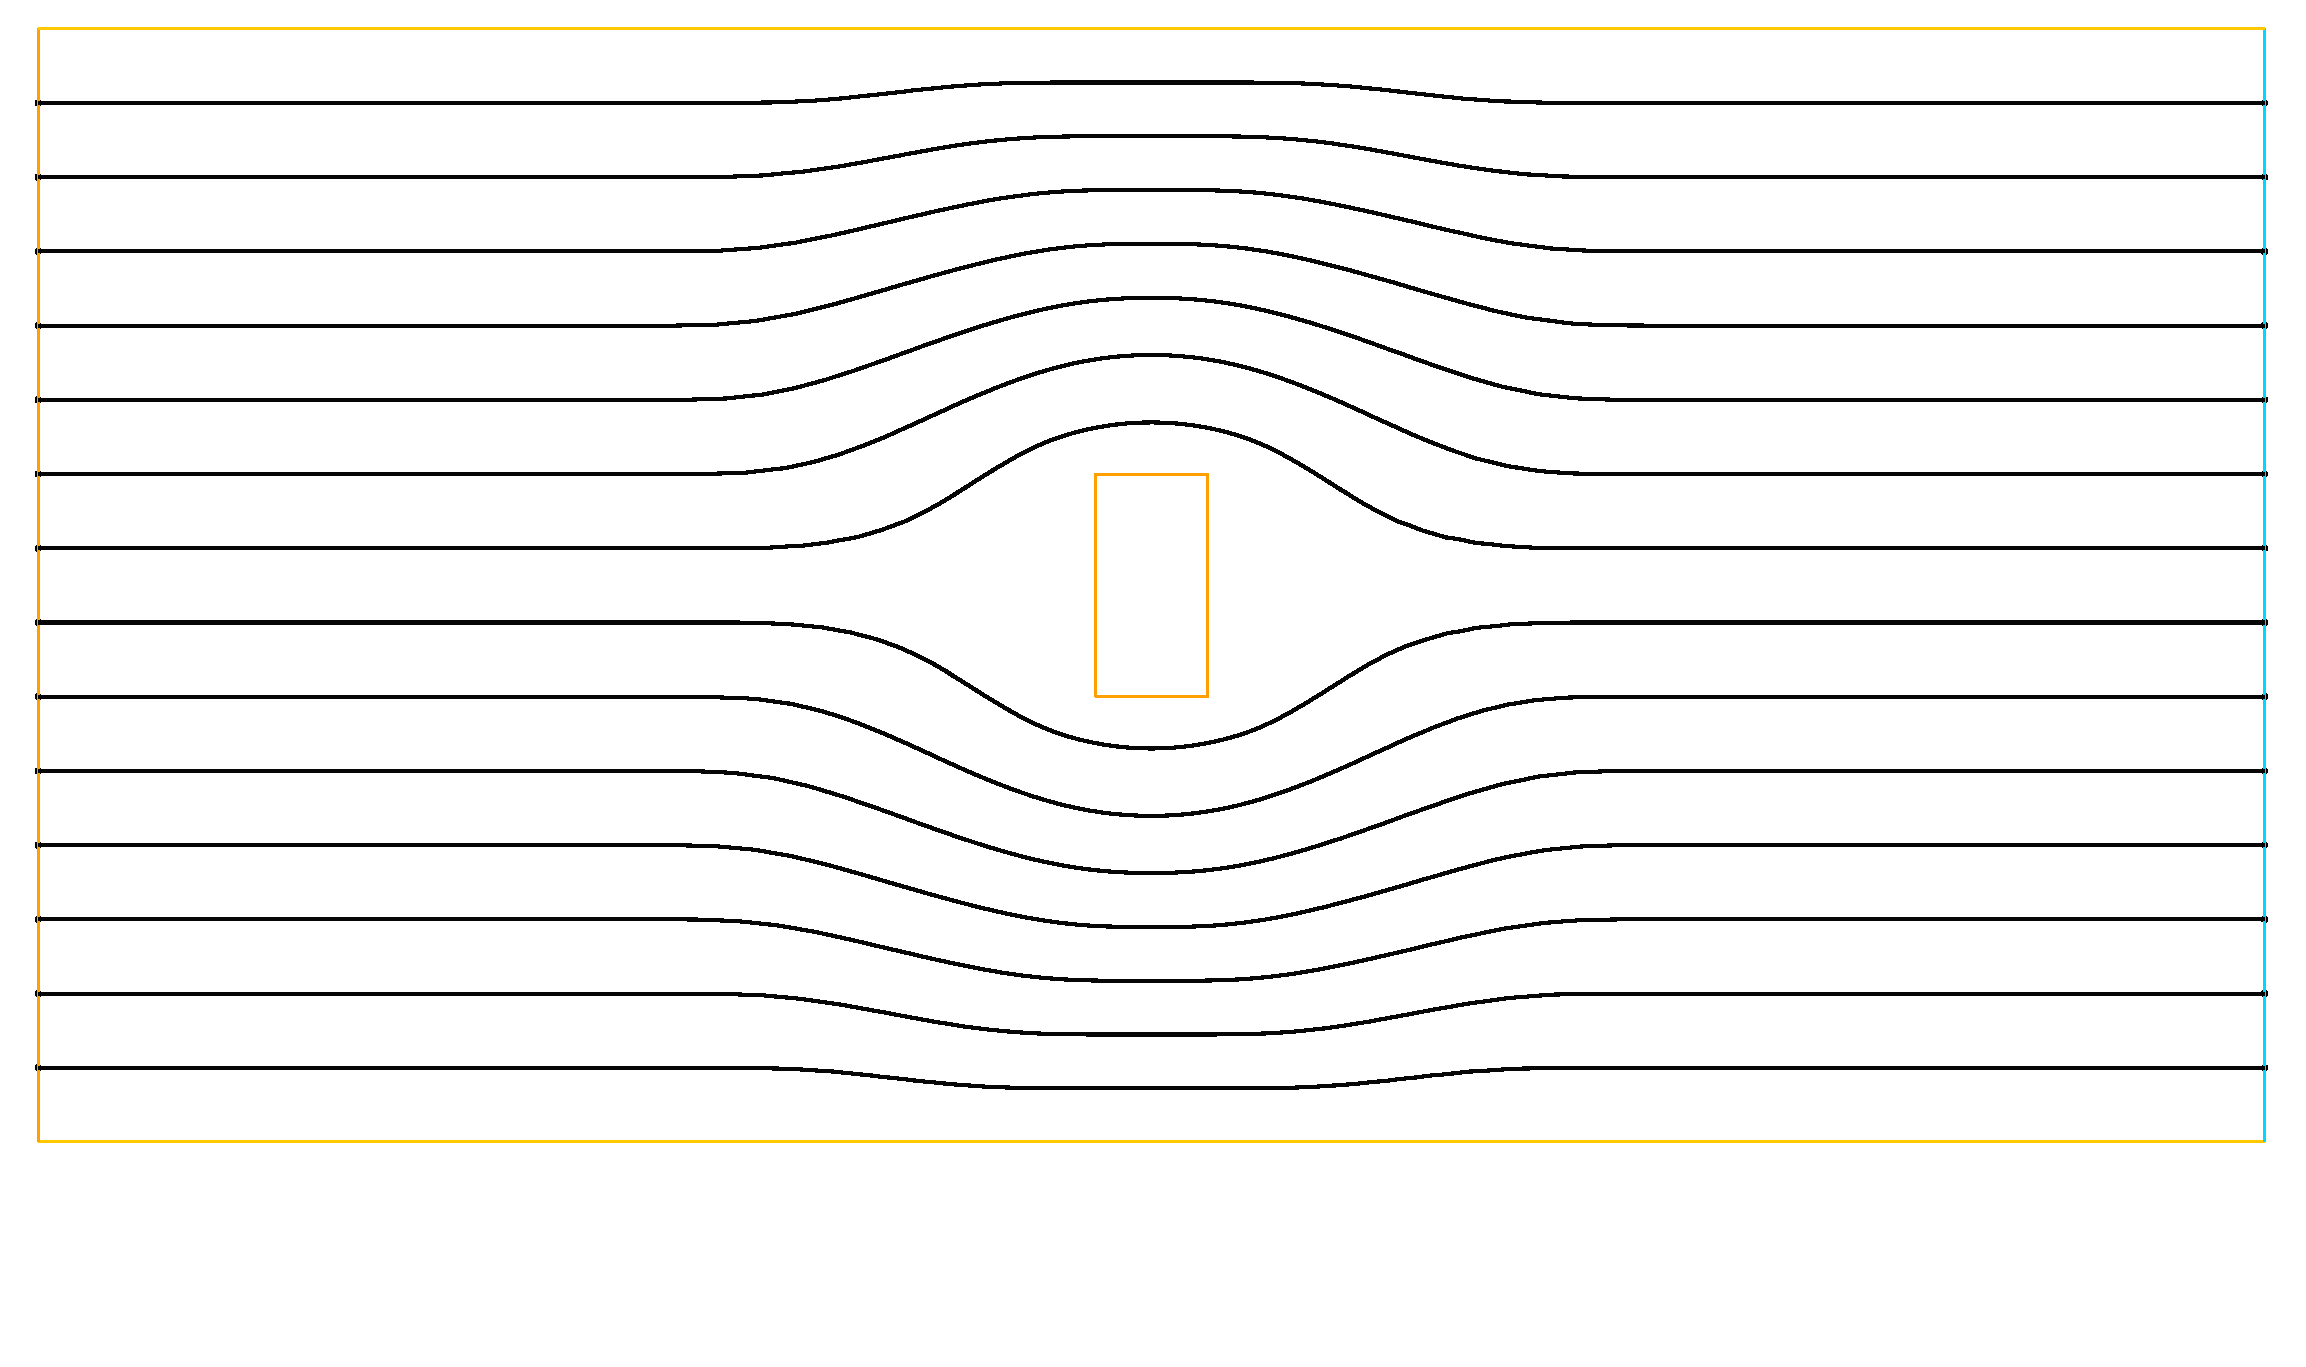
\includegraphics[width=0.9\textwidth]{../figures/cylinder_overview_empty.pdf}
            }
            \only<2>{
                \centering
                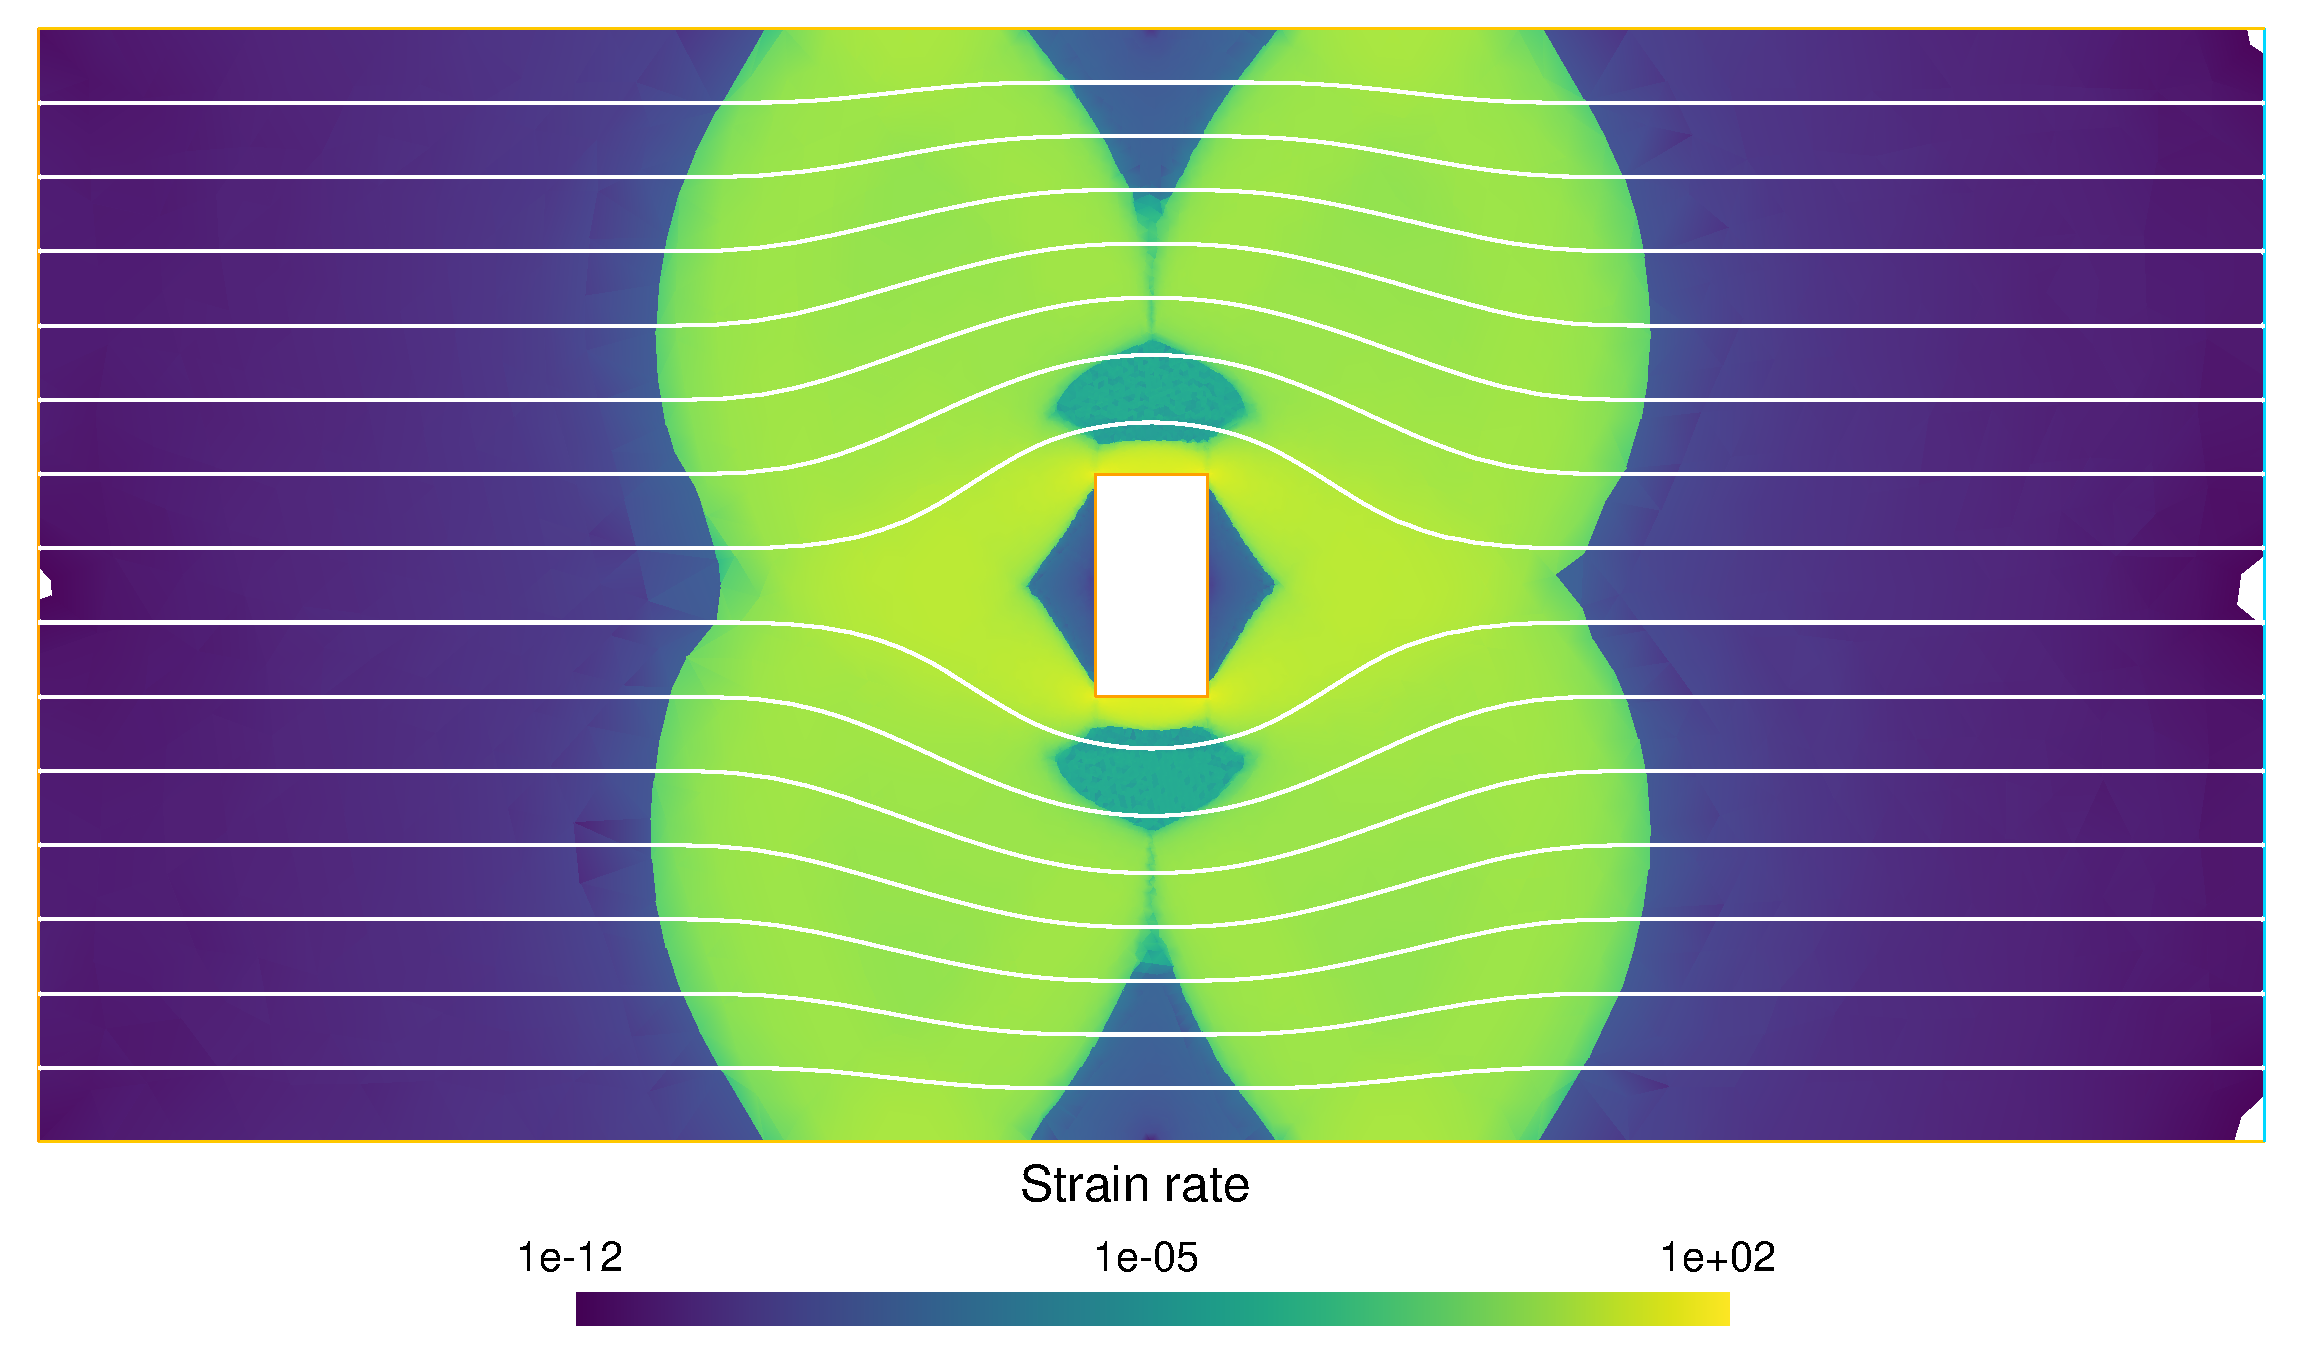
\includegraphics[width=0.9\textwidth]{../figures/cylinder_overview.pdf}
            }
        \end{overprint}
    \end{figure}
\end{frame}

\begin{frame}{Flow around an obstacle - Rigid body motion}
    \begin{figure}
        \centering
        \movie[width=0.725\textheight, height=0.75\textheight, autostart, loop]{} {../anim/obstacle/obstacle_arrows.mp4}
    \end{figure}
\end{frame}

%---------------------------------------------------------

\section{Improvements}
\begin{frame}{Corners of rigid regions}
    \begin{figure}
        \begin{overprint}
            \only<1>{
                \centering
                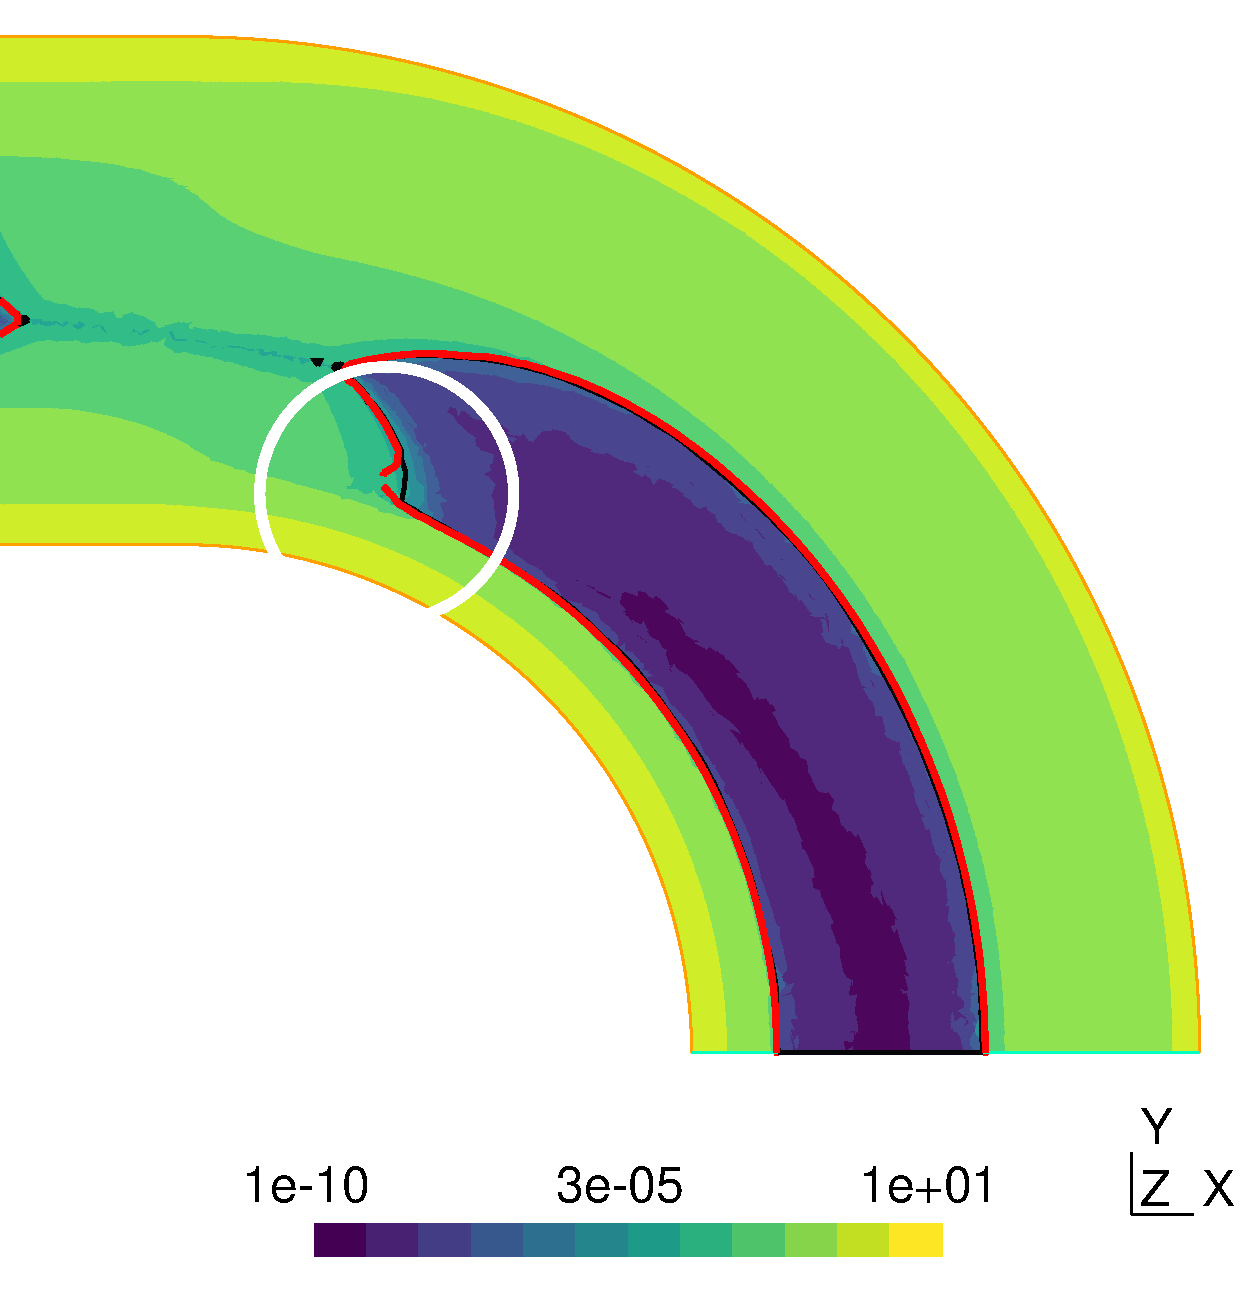
\includegraphics[height=0.65\textheight]{../figures/corner_5.pdf}
                \caption*{Strain rate of the flow in a curved channel}
            }
            \only<2>{
                \centering
                \includesvg[height=0.65\textheight]{../figures/corner_4.svg}
                \caption*{Virtual field $\phi$, interface predictor/corrector in black/red.}
            }
        \end{overprint}
    \end{figure}
\end{frame}

\begin{frame}{Corners of rigid regions}
    \begin{figure}
        \centering
        \begin{subfigure}[t]{0.26\textwidth}
            \includesvg[width=\textwidth]{../figures/corner_1.svg}
        \end{subfigure}
        \begin{subfigure}[t]{0.26\textwidth}
            \includesvg[width=\textwidth]{../figures/corner_2.svg}
        \end{subfigure}
        \begin{subfigure}[t]{0.26\textwidth}
            \includesvg[width=\textwidth]{../figures/corner_3.svg}
        \end{subfigure}
        \caption*{Successive linear approximations around the interface predictor}
    \end{figure}
\end{frame}

\begin{frame}{Yield tolerance parameter}
    \begin{itemize}
        \item $\dot\gamma(\vv^h)$ never exactly $0$, but from $\sim 10^{-12}$ to $\sim 10^{-5}$
        \item Interface predictor selects elements with $\dot\gamma(\vv^h)<10^{-4}$
        \item Would prefer algorithm predicts interface autonomously
    \end{itemize}
\end{frame}

\begin{frame}{Yield tolerance parameter}
    \begin{figure}
        \begin{overprint}
            \only<1>{
                \centering
                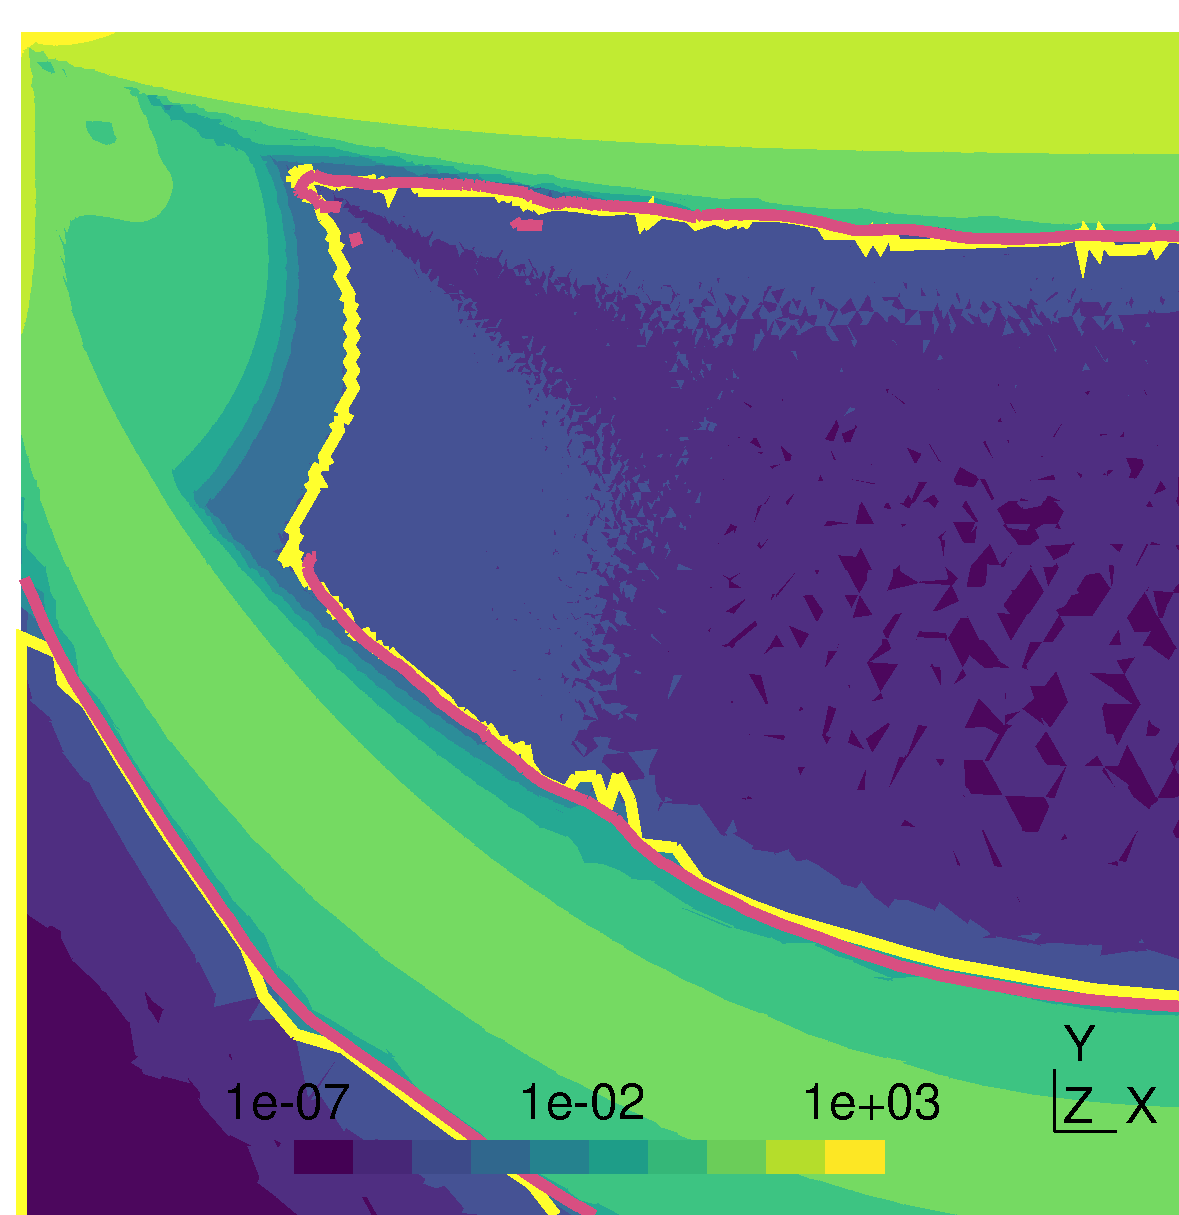
\includegraphics[height=0.65\textheight]{../figures/correction_1.pdf}
                \caption*{Strain rate of the lid-driven cavity flow, predictor/corrector in yellow/red}
            }
            \only<2>{
                \centering
                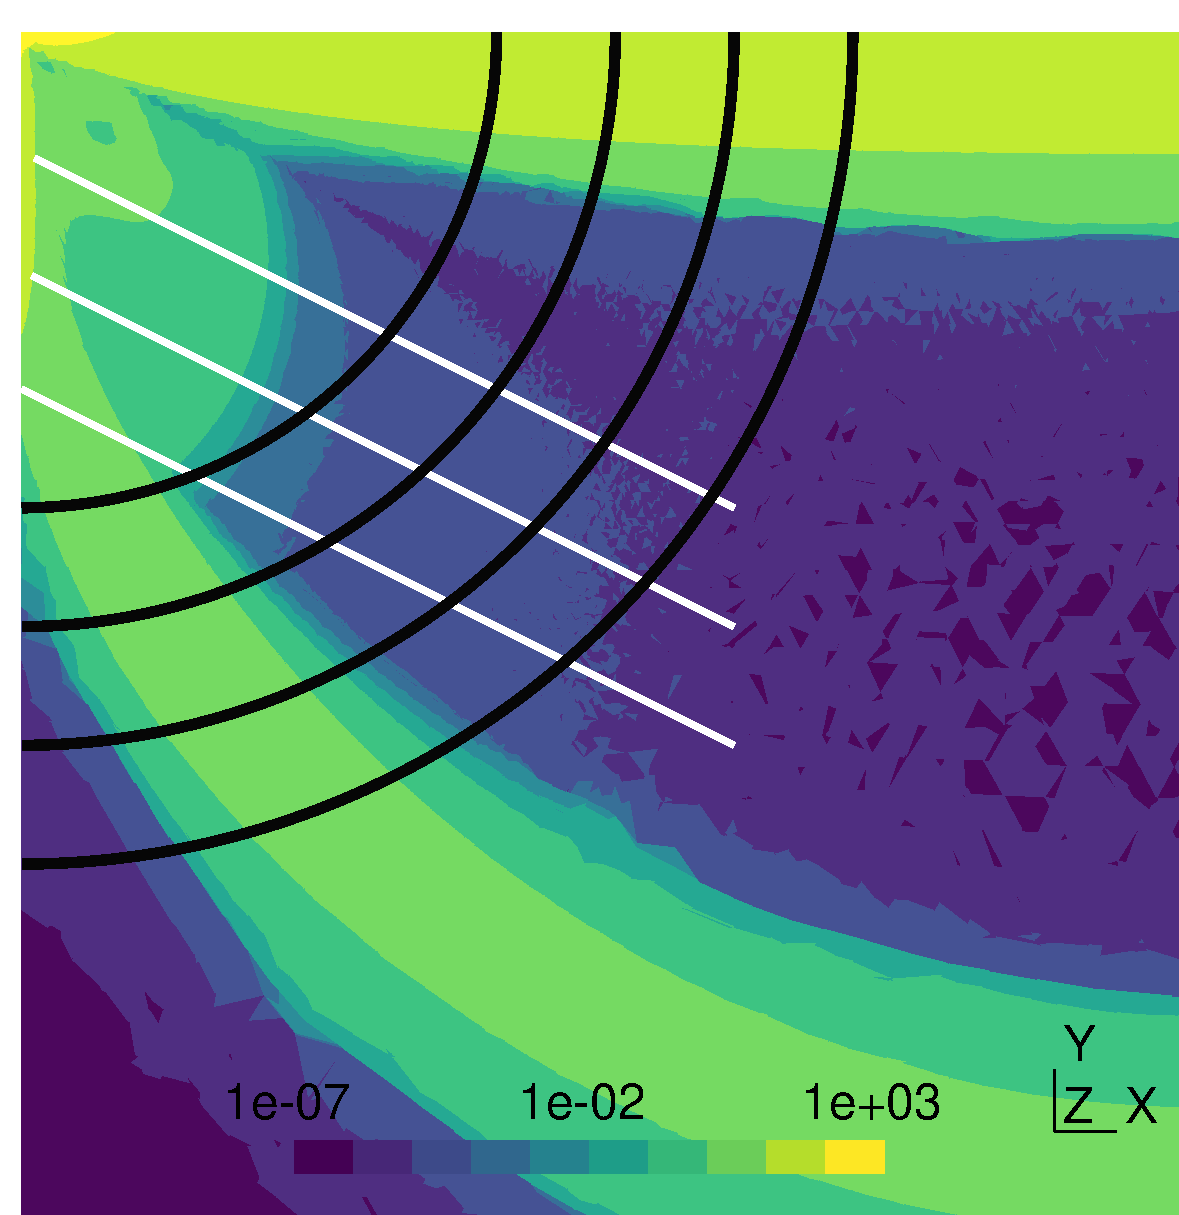
\includegraphics[height=0.65\textheight]{../figures/correction_2.pdf}
                \caption*{Parametric curves}
            }
        \end{overprint}
    \end{figure}
\end{frame}

\begin{frame}{Yield tolerance parameter}
    \begin{figure}
        \begin{overprint}
            \only<1>{
                \centering
                \includesvg[width=0.9\textwidth]{../figures/correction_4.svg}
            }
            \only<2>{
                \centering
                \includesvg[width=0.9\textwidth]{../figures/correction_3.svg}
            }
        \end{overprint}
        \caption*{Evaluation of the strain rate along the parametric curves}
    \end{figure}
\end{frame}

\section*{}
\begin{frame}
    \begin{center}
        \LARGE
        Thank you for your attention !
        \normalsize
    \end{center}
    \begin{figure}
        \centering
        \movie[width=0.71\textheight, height=0.6\textheight, autostart, loop]{} {../anim/obstacle/cropped.mp4}
    \end{figure}
\end{frame}
%---------------------------------------------------------

\end{document}



% \begin{frame}{Governing equations}
%     \begin{equation*}
%     \begin{aligned}
%         \nabla \cdot \boldsymbol\sigma + \mathbf{f} &= \mathbf{0}\\
%         \nabla \cdot \uu &= 0
%     \end{aligned}
%     \end{equation*}
    
%     \begin{equation*}
%     \begin{aligned}
%         &\;\;\: \mathbf{d} = \frac{1}{2} (\nabla u + \nabla u^T)\\
%         &\begin{cases}
%             \mathbf{s} = 2 \mu \mathbf{d} + 2 \tau_0 \frac{\mathbf{d}}{\|\mathbf{d}\|} & \text{if} \sqrt{\frac{1}{2}\mathbf{s}:\mathbf{s}} \geq \tau_0\\
%             \mathbf{d} = \mathbf{0} & \text{if} \sqrt{\frac{1}{2}\mathbf{s}:\mathbf{s}} \leq \tau_0\\
%         \end{cases}\\
%         &\;\;\: \uu = \uu \quad \text{on} \quad \partial \Omega
%     \end{aligned}
%     \end{equation*}
% \end{frame}


% \begin{frame}{Minimum principle}
%     \begin{align*}
%         \uu = \text{arg} \min_{\vv \in \mathcal{V}} \; \frac{1}{2}\int_{\Omega} \mu \|\mathbf{d}\|^2 \dd{\Omega} + \int_{\Omega} \tau_0 \|\mathbf{d}\| \dd{\Omega} - \int_{\Omega} \mathbf{f} \cdot \vv \dd{\Omega}
%     \end{align*}
    
%     \vspace{1cm} 
%     How do they obtain it ? Multiply by a test function \& integrate ? But how did they handle the discontinuity of the stress tensor ?
% \end{frame}

% \begin{frame}{Finite element discretization}
%     \begin{align*}
%         \vv_h(\xx) &= \sum_{i=1}^{n} N_i(\boldsymbol \xi) \vv_i
%     \end{align*}
%     \begin{align*}
%         \mathbf{d}_h(\xx) &=
%         \begin{bmatrix}
%             d_{xx}\\
%             d_{yy}\\
%             d_{xy}
%         \end{bmatrix} = \mathbf{J}_e^{-T} 
%         \begin{bmatrix}
%             N_{1, \xi} & 0 & N_{2, \xi} & 0 & \dots & N_{n, \xi} & 0\\
%             0 & N_{1, \eta} & 0 & N_{2, \eta} & \dots & 0 & N_{n, \eta}\\
%             N_{1, \eta} & N_{1, \xi} & N_{2, \eta} & N_{2, \xi} & \dots & N_{n, \eta} & N_{n, \xi}
%         \end{bmatrix} \vv_i\\
%     \end{align*}
    
%     \begin{itemize}
%         \item How can the Jacobian be 3x3 with a 2D problem ?
%         %\item With linear shape functions, the "matrix of derivatives" is constant.
%     \end{itemize}
% \end{frame}

% \begin{frame}{Minimization formulation}
%     Define $Q$ to easily evaluate $\|\mathbf{d}\| = \sqrt{2 \mathbf{d}: \mathbf{d}} \quad \longrightarrow \quad \mathbf{Q} = \textrm{diag}(2, 2, 1)$.
    
%     Using a Gaussian quadrature with $N_g$ integration points and weights $\omega_g$:
%     \begin{align*}
%         J(\vv) = \sum_{e=1}^{N_e} \sum_{g=1}^{N_g} \omega_g \det \mathbf{J}_e \left(\frac{\mu}{2} \Big\|\mathbf{Q} \mathbf{d}_h(\xx_g)\Big\|^2 + \tau_0 \Big\|\mathbf{Q} \mathbf{d}_h(\xx_g)\Big\| + \right) - \mathbf{f}^T \cdot \vv
%     \end{align*}

%     \begin{equation*}
%     \begin{aligned}
%         \implies \min_{\vv} \quad& J(\vv)\\
%         \text{s.t.} \quad& d_{xx} + d_{yy} = 0\\
%                       & \vv_I = \uu^d\\
%     \end{aligned}
%     \end{equation*}
    
%     \begin{itemize}
%         \item $\mathbf{f}^T \cdot \vv$ is the discrete version of $\int_{\Omega} \mathbf{f}(\xx) \cdot \vv(\xx) \dd{\Omega}$
%     \end{itemize}
% \end{frame}

% \begin{frame}{Conic optimization}
%     \begin{itemize}
%         \item Linear objective
%         \item Linear constraints
%         \item "Special constraints", or cones $$ \text{Let } K \subseteq \mathbb{R}^n \qquad x \succcurlyeq 0 \iff x \in K$$
%     \end{itemize}
    
%     \vspace{1cm}
%     Generalization of "classic" inequalities:
%     \begin{align*}
%         a \succcurlyeq b \iff a-b \succcurlyeq 0 \iff a-b \in K\\
%     \end{align*}
% \end{frame}

% \begin{frame}{Proper cones: properties to satisfy}
%     \begin{enumerate}
%         \item $a \succcurlyeq 0 \implies \lambda a \succcurlyeq 0$ for $\lambda \in \mathbb{R}^+$ (Cone)
%         \item $a \succcurlyeq 0$ and $b \succcurlyeq 0 \implies a+b \succcurlyeq 0$ (Closed under addition)
%         \item $x \succcurlyeq 0$ and $x \preccurlyeq 0 \implies x = 0$ (Pointed)
%         \item $\textrm{int} (K) \neq \emptyset$ (Solid)
%         \item $\{x_i\}_{i\to\infty}$ with $x_i \succcurlyeq 0$ then $\lim_{i} x_i = \bar x$ with $\bar x \succcurlyeq 0$  (Closed)
%     \end{enumerate}
% \end{frame}

% \begin{frame}{Examples (1)}
%     \begin{itemize}
%         \item \textbf{In 1D}, only $\emptyset$, $\mathbb{R}^+$, $\mathbb{R}^-$.
    
%         \item \textbf{In 2D}, only "linear" cones: $\emptyset$, and regions between two half lines with an angle less than 180 degrees.
%     \end{itemize}
%     \pause
%     \begin{figure}
%         \centering
%         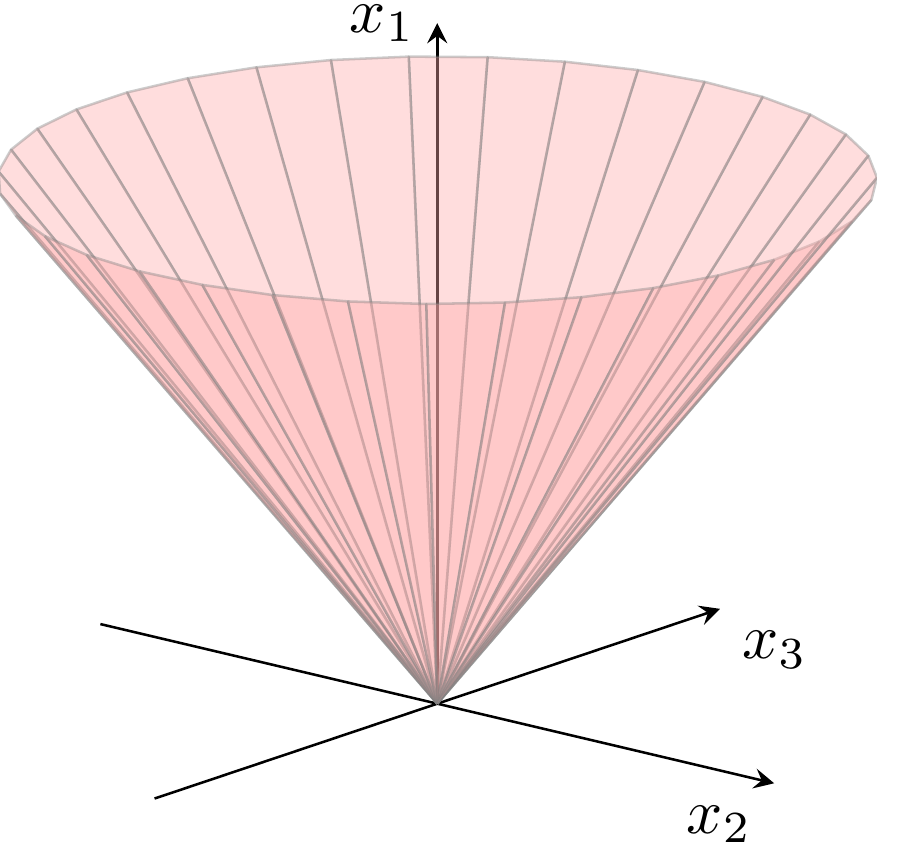
\includegraphics[width=0.4\textwidth]{../docs/Cone_Lorentz.png}
%         \label{fig:2d_cone}
%     \end{figure}
    
% \end{frame}

% \begin{frame}{Examples (2)}
%     \begin{itemize}
%         \item Lorentz cone $$\mathbb{L}^n = \{\xx \in \mathbb{R}^{n+1} \big\vert x_1 \geq \sqrt{x_2^2+x_3^2+\dots + x_{n+1}^2}\}$$
%         \begin{figure}
%             \centering
%             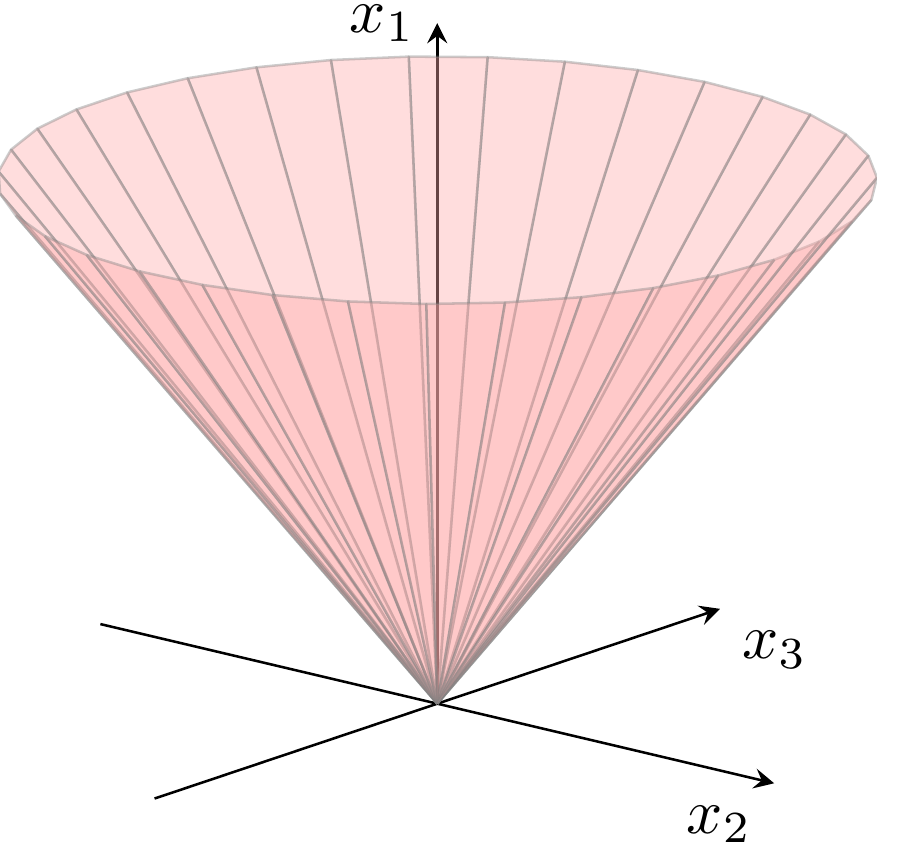
\includegraphics[height=0.4\textheight]{../docs/Cone_Lorentz.png}
%             \caption{https://docs.mosek.com/modeling-cookbook/\_images/qcone.png}
%             \label{fig:Lorentz_cone}
%         \end{figure}
%     \end{itemize}
% \end{frame}

% \begin{frame}{Examples (3)}
%     \begin{itemize}
%         \item Exponential cone $$\mathbb{E} = \textrm{closure}\left\{(x, y, z) \in \mathbb{R}^{3} \;\big\vert\; z \geq y \exp\left(\frac{x}{y}\right) \text{ and } y>0 \right\}$$
%         \begin{figure}
%             \centering
%             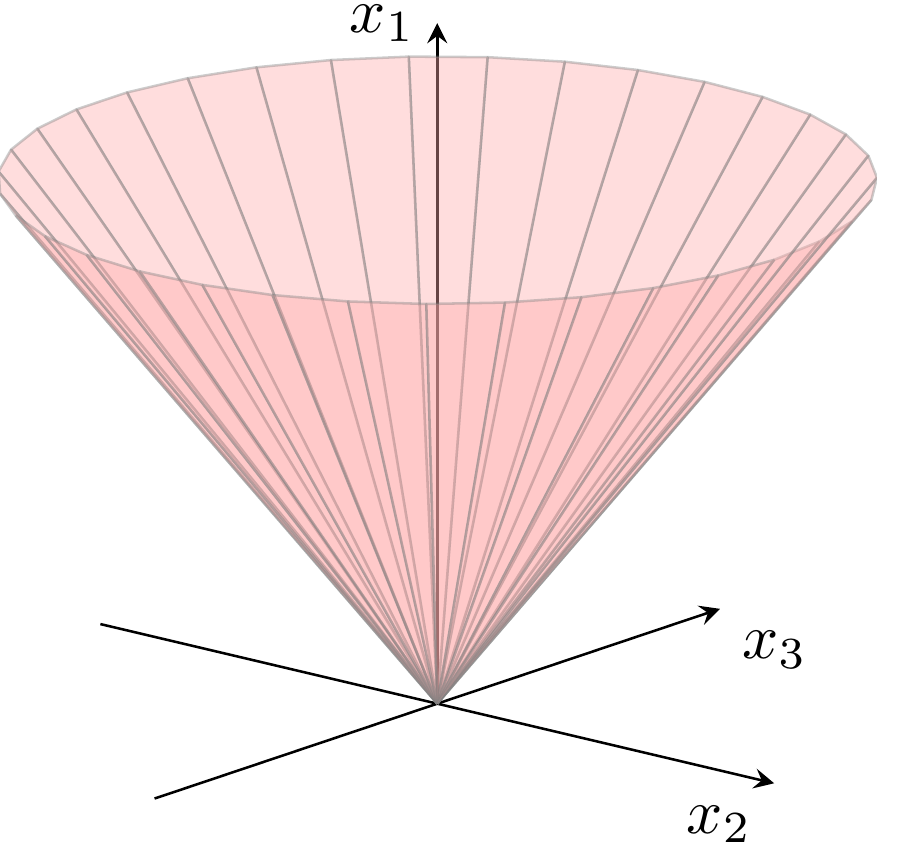
\includegraphics[height=0.4\textheight]{../docs/Cone_Lorentz.png}
%             %\caption{https://docs.mosek.com/modeling-cookbook/\_images/expcone.png}
%             \label{fig:Exp_cone}
%         \end{figure}
%     \end{itemize}
% \end{frame}

% \begin{frame}{Examples (4)}
%     \begin{itemize}
%         \item Power cone, with $0 < a < 1$ $$\mathbb{P}_{\alpha} = \left\{(x, y, z) \in \mathbb{R}^{3} \;\big\vert\; |z| \leq x^{\alpha} y^{1-\alpha},\: x>0,\: y>0\right\}$$
%         \begin{figure}
%             \centering
%             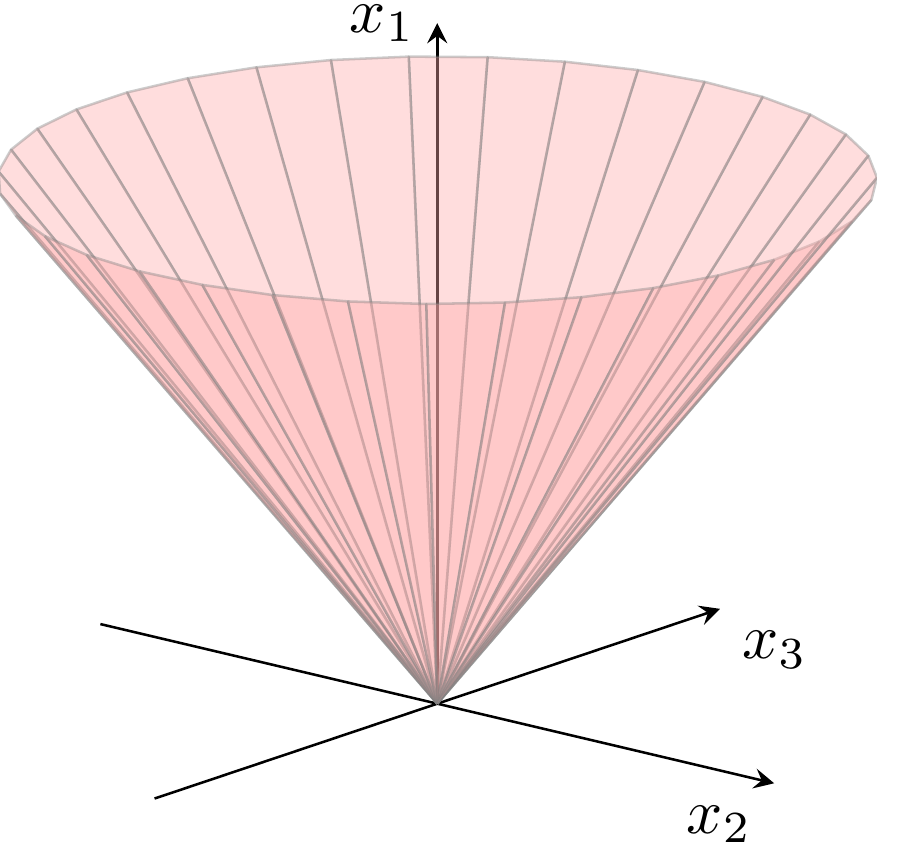
\includegraphics[height=0.65\textheight]{../docs/Cone_Lorentz.png}
%             %\caption{https://docs.mosek.com/modeling-cookbook/\_images/powcone.png}
%             \label{fig:Power_cone}
%         \end{figure}
%     \end{itemize}
% \end{frame}

% \begin{frame}{Examples (5)}
%     \begin{overprint}
%     \onslide<1>
%     \begin{itemize}
%         \item Semidefinite cone for SPD matrices
%         \item Others, but most important one covered
%     \end{itemize}
%     \onslide<2->
%     \begin{figure}
%         \centering
%         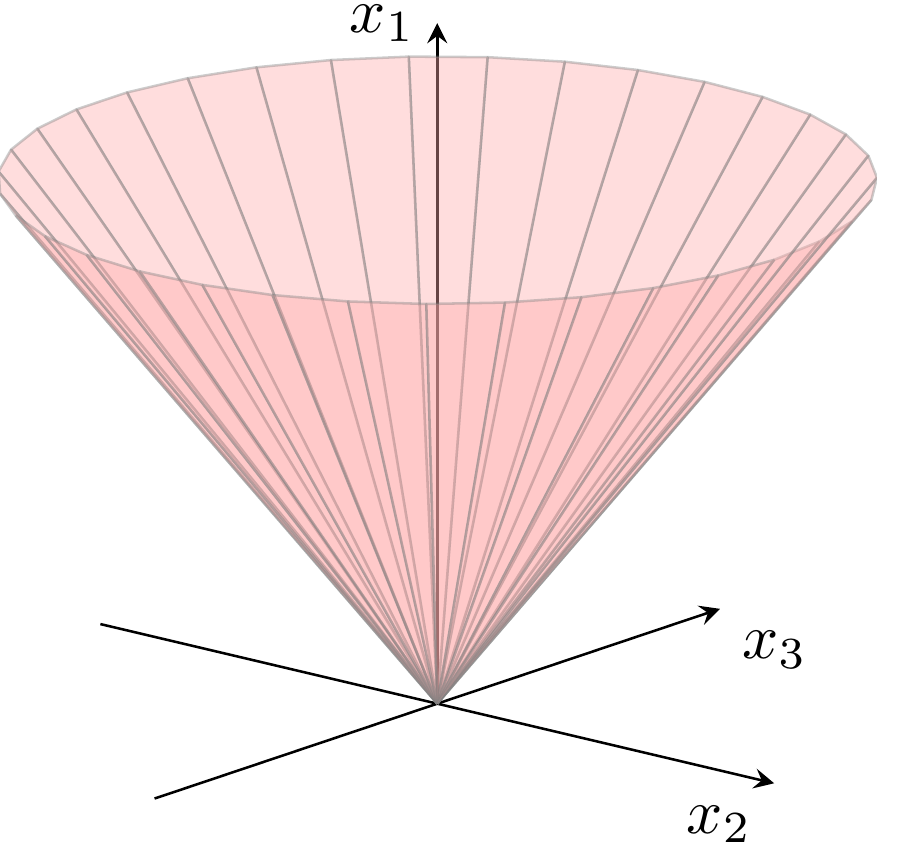
\includegraphics[height=0.8\textheight]{../docs/Cone_Lorentz.png}
%         %\caption{https://docs.mosek.com/cheatsheets/conic.pdf}
%         \label{fig:Cheatsheet}
%     \end{figure}
%     \end{overprint}
% \end{frame}


% \begin{frame}{Rotated cone (1)}
%     \begin{align*}
%         \mathbb{L}_R^n = \{(\xx, y, z) \in \mathbb{R}^{n}\times\mathbb{R}\times\mathbb{R} \;\big\vert\; 2  y z &\geq x_1^2 + x_2^2+\dots + x_n^2\}\\
%         \frac{(y+z)^2}{2}&\geq \frac{(y-z)^2}{2} + x_1^2+\dots +x_n^2\\
%         \frac{(y+z)}{\sqrt{2}}&\geq \sqrt{\left(\frac{y-z}{\sqrt{2}}\right)^2 + x_1^2+\dots +x_n^2}
%     \end{align*}
%     \begin{itemize}
%         \item Which is equivalent to say that $\left(\frac{y+z}{\sqrt{2}}, \frac{y-z}{\sqrt{2}}, \xx \right) \in \mathbb{L}^{n+1}$.
%     \end{itemize}
% \end{frame}

% \begin{frame}{Rotated cone (2)}
%     \begin{figure}
%         \centering
%         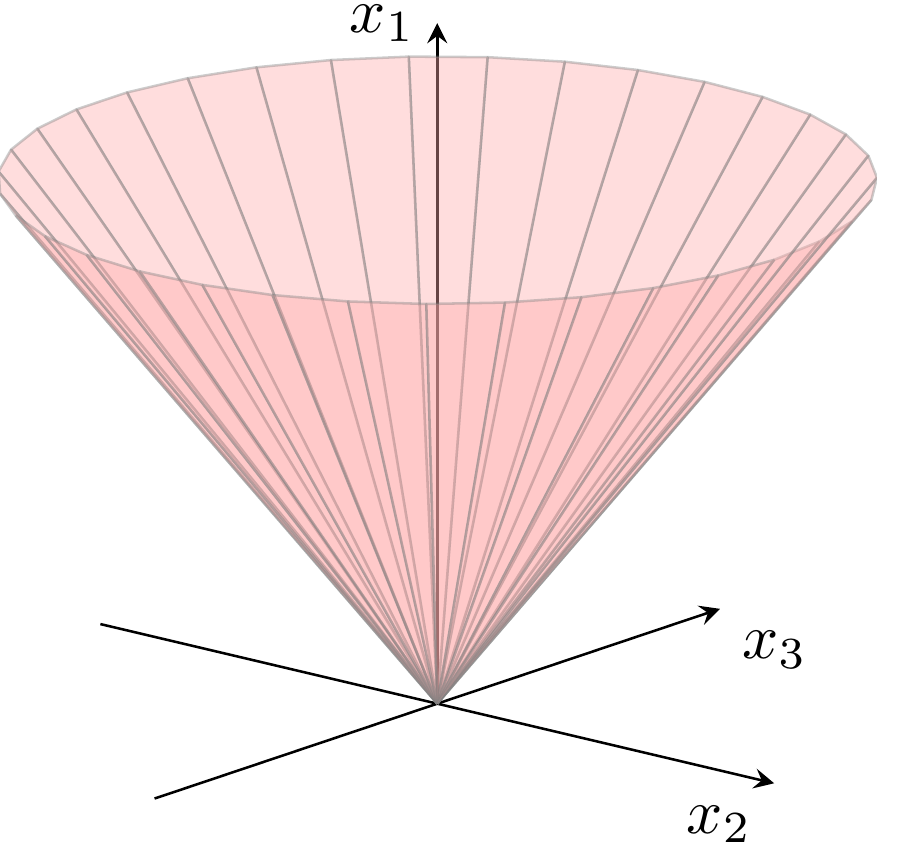
\includegraphics[height=0.4\textheight]{../docs/Cone_Lorentz.png}
%         \label{fig:Rot_Lorentz_cone}
%     \end{figure}
% \end{frame}

% \begin{frame}{Why so strong ?}
%     \begin{itemize}
%         %\item \textbf{Dual formulation} as with linear programming (bounds). However, harder now because cones are not always self-dual.
%         \item For every proper cone, there exists a \textbf{self-concordant barrier}: very useful functions that give a perfect framework for \textbf{Newton's method}. 
%         $$g \text{ is convex and } \quad |g'''(x)| \leq 2 g''(x) ^ {3/2}$$
%         They ensure \textbf{global convergence} of NR, no erratic behavior possible.
%         \item \textbf{Interior-point method}: all constraints $g$ are moved into an objective function $f_{obj}$ and multiplied by $\mu \to 0$: $$f_{obj} = \textrm{linear objective} + \mu \sum\textrm{Barrier functions}$$
%         %\item Estimated distance to optimal solution : $\delta^2(\mathbf x) = \nabla f^T (\nabla^2 f)^{-1} \nabla f$. If iterate $x_i$ "close" from $x^*$: quadratic convergence ! Otherwise, we "damp" the steps.
%         \item Solution obtained with accuracy $\epsilon$ after $\mathcal{O}\left(\sqrt{\nu} \log \frac{1}{\epsilon}\right)$ iterations, where $\nu=\sum\nu_i$, where $\nu_i$ is the parameter of the barrier $i$.
%     \end{itemize}
% \end{frame}

% \begin{frame}{2D example of Interior-point method: min(x)}
% %    \begin{figure}
% %    \centering
% %    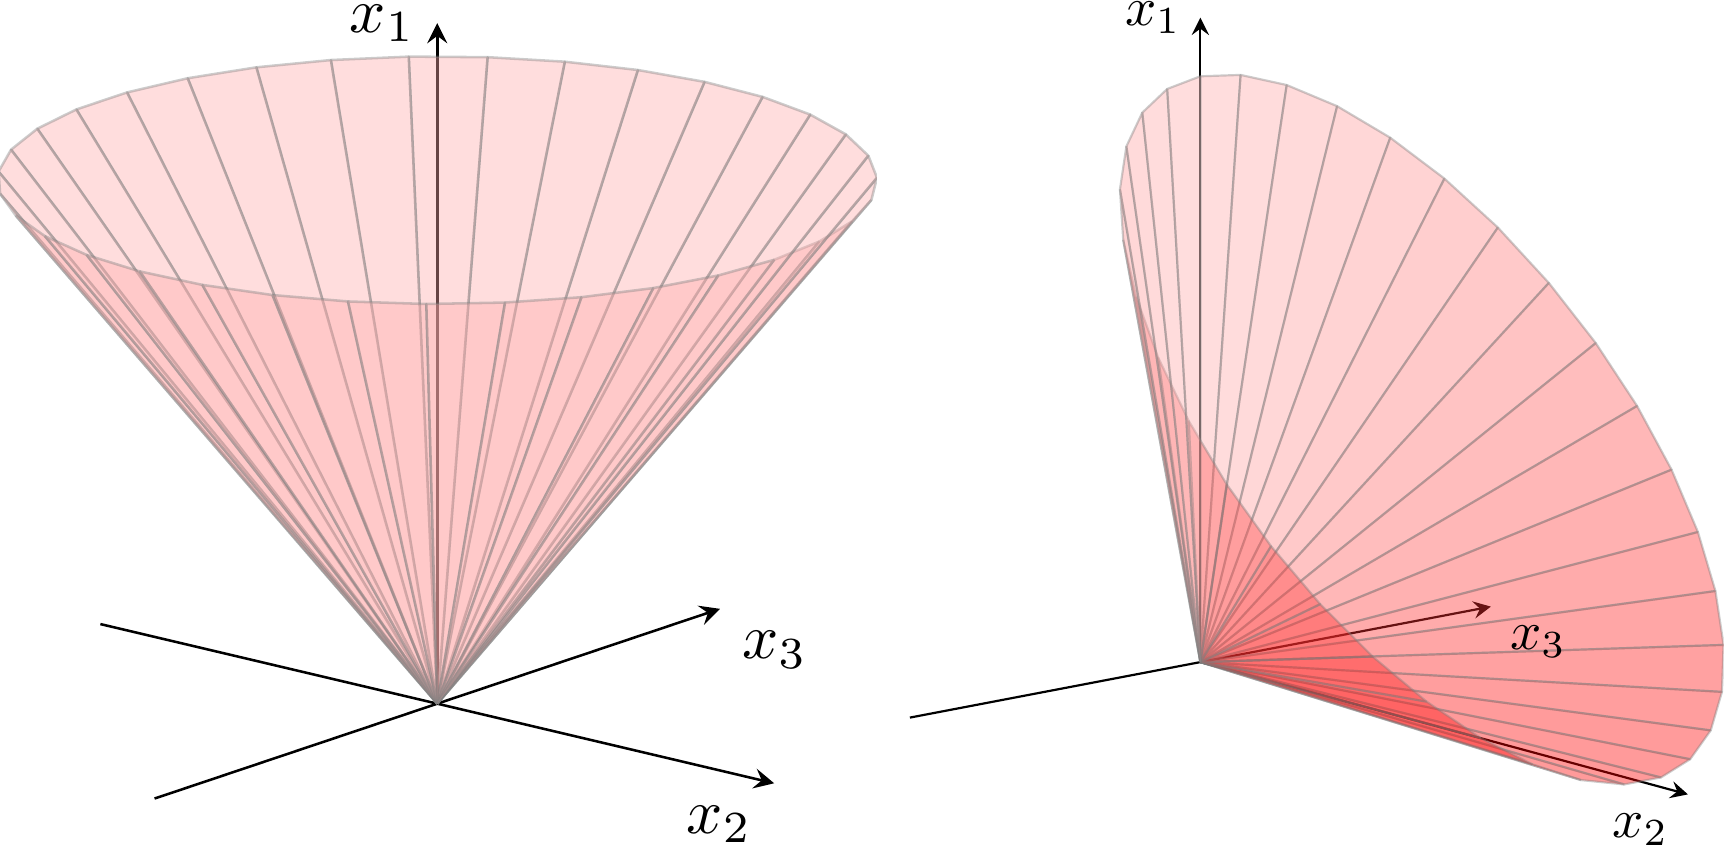
\includegraphics[height=0.4\textheight]{Figures/Lorentz_cone_rot.png}
% %    \label{fig:Rot_Lorentz_cone}
% %    \end{figure}
%     \begin{overprint}
%     \onslide<1>\centering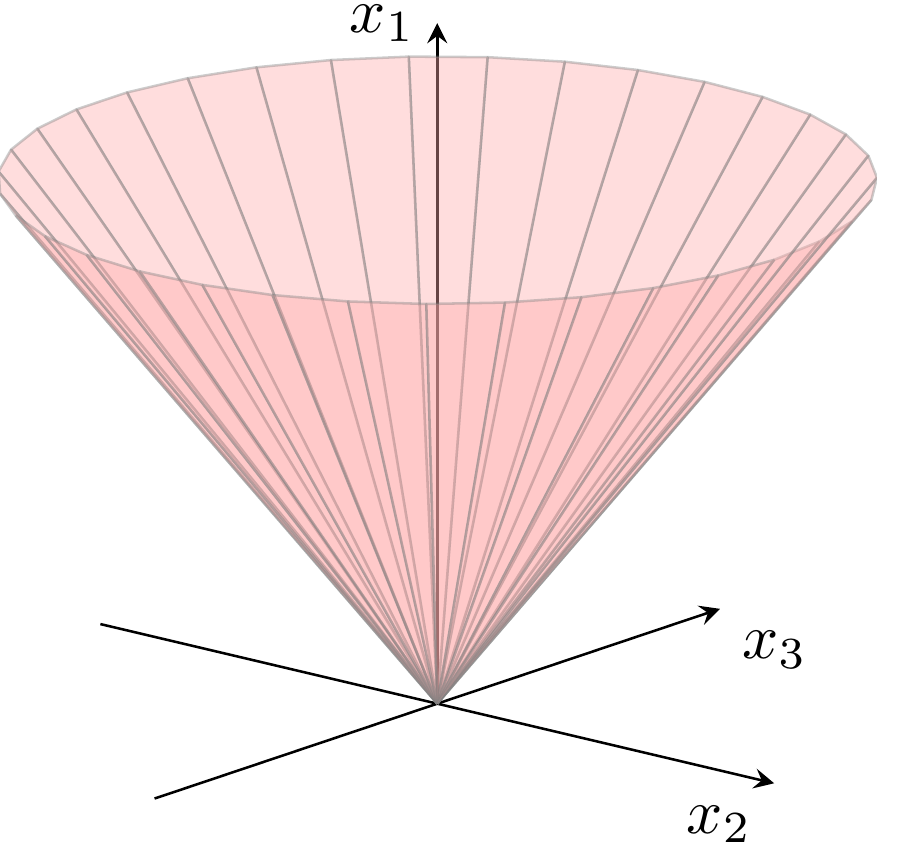
\includegraphics[height=0.7\textheight]{../docs/Cone_Lorentz.png}\\$\mu \gg 1$
%     \onslide<2>\centering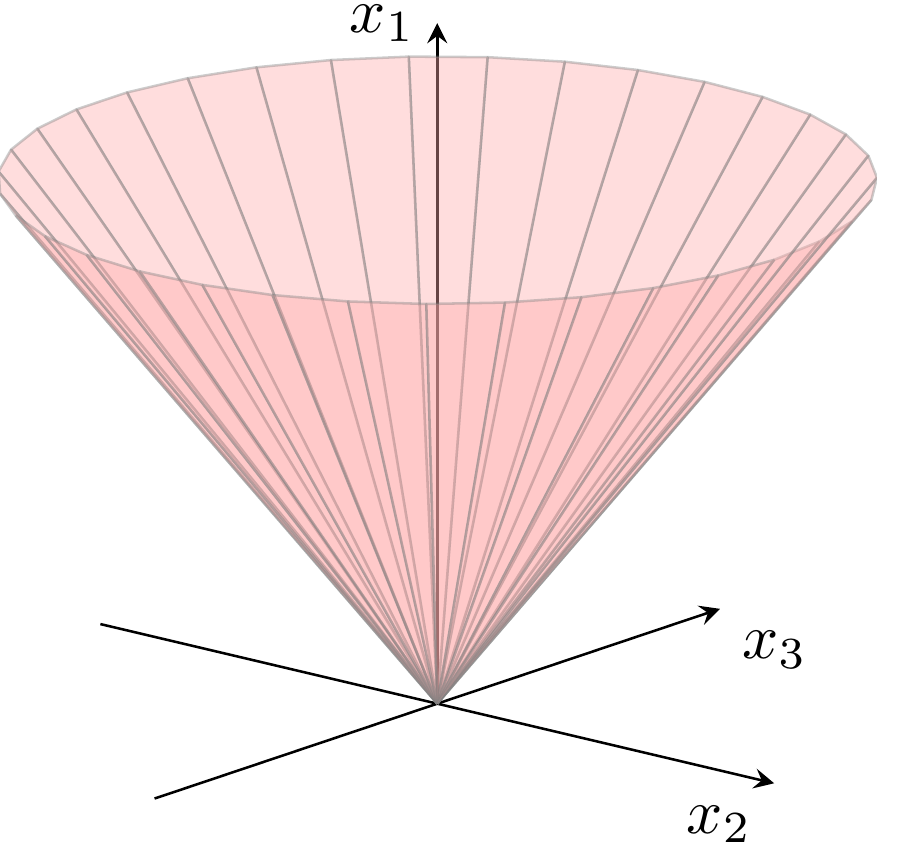
\includegraphics[height=0.7\textheight]{../docs/Cone_Lorentz.png}\\$\mu \approx 1$
%     \onslide<3->\centering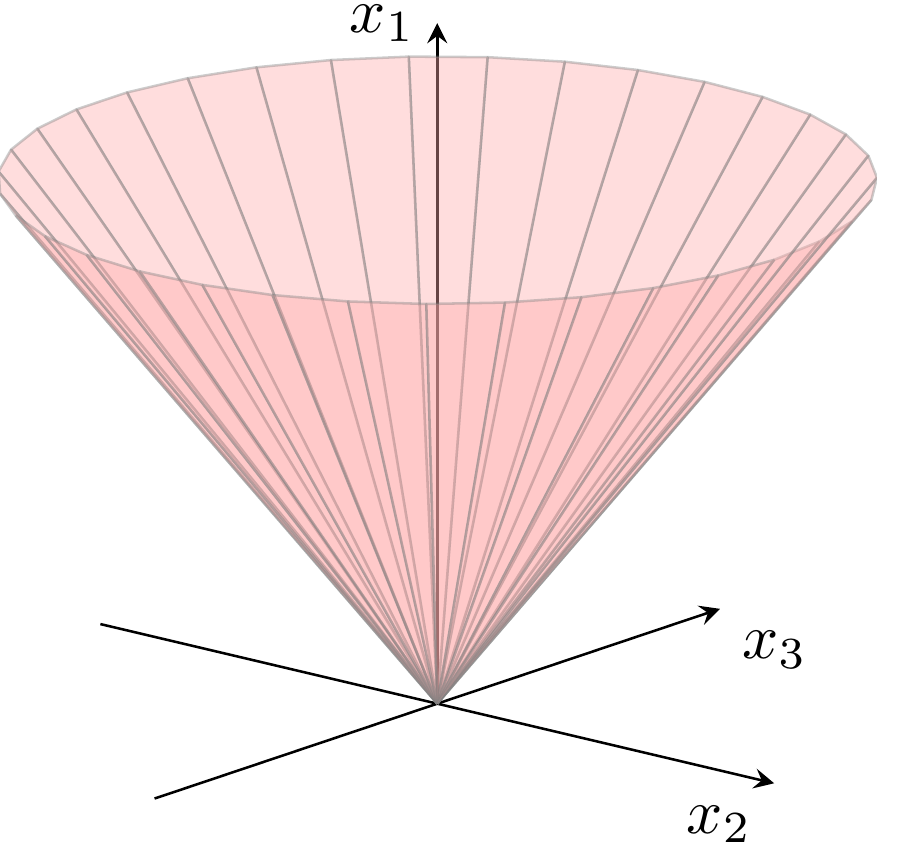
\includegraphics[height=0.7\textheight]{../docs/Cone_Lorentz.png}\\$\mu \ll 1$
%     \end{overprint}
% \end{frame}

% \begin{frame}{Back to yield-stress fluid flow... in 1D}
%     \begin{itemize}
%         \item 1D $\implies \nabla \cdot \vv=0$ automatically satisfied with $\vv = u(y)$
%         \item Linear shape functions $\implies$ only 1 integration point needed
%         \item $\det \mathbf{J}_e = \Delta y$, and $\|\mathbf{d}\| = \left|\pdv{u}{y}\right| = \left| \frac{\Delta u}{\Delta y}\right|$
%     \end{itemize}
    
%     \begin{align*}
%         \min_{u} \quad &\sum_e \frac{\mu}{2 \Delta y} \|\Delta u\|^2 + \tau_0 \|\Delta u\| - \mathbf{f} \cdot \uu\\
%         \iff \qquad \min_{u} \quad& \sum_e \frac{\mu}{2 \Delta y} s_e + \tau_0 t_e - \mathbf{f} \cdot \uu\\
%         \text{s.t.} \quad& \|\Delta u\|^2 \leq s_e \:\;\iff\quad (0.5, s_e, u_{e+1}-u_e) \in \mathbb{L}_R^1 \\
%         &\|\Delta u\| \leq t_e \quad\iff\quad (t_e, u_{e+1}-u_e) \in \mathbb{L}^1 \\
%         & u_0 = u_{N_e} = 0
%     \end{align*}
    
%     \begin{itemize}
%         \item Bounds are tight at the optimum. This reformulation is possible because the coefficients of $\|\Delta u\|^2$ and $\|\Delta u\|$ are positive.
%     \end{itemize}
% \end{frame}

% \begin{frame}{Canonical form (for the Python code)}
%     \begin{align*}
%         \min \quad& c^T x\\
%         \text{s.t.} \quad& A x = b\\
%         & Gx + s = h\\
%         & s \succcurlyeq 0
%     \end{align*}
    
%     \begin{align*}
%         \xx &= 
%         \begin{bmatrix}
%             \uu & \mathbf{s} & \mathbf{t}
%         \end{bmatrix}\\
%         \mathbf{c} &= 
%         \begin{bmatrix}
%             \boldsymbol -\mathbf{f} & \frac{\mu}{2\Delta y \vert_e} & \tau_0
%         \end{bmatrix}\\
%         \mathbf{G} &= \dots\\
%         \mathbf{h} &= \dots
%     \end{align*}
% \end{frame}

% \begin{frame}{Numerical Simulation}
%     \begin{overprint}
%     \onslide<1>
%         \begin{figure}
%             \centering
%             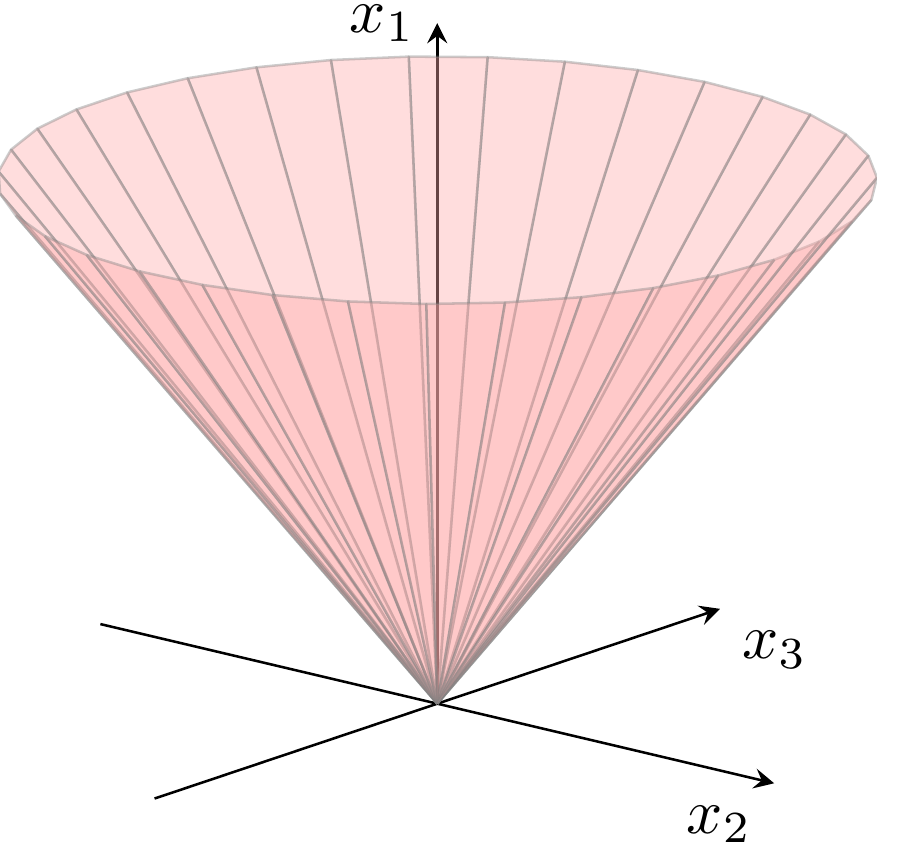
\includegraphics[width=0.4\textwidth]{../docs/Cone_Lorentz.png}
%             \caption{Arbitrary Mesh}
%         \end{figure}
%     \onslide<2>
%         \begin{figure}
%             \centering
%             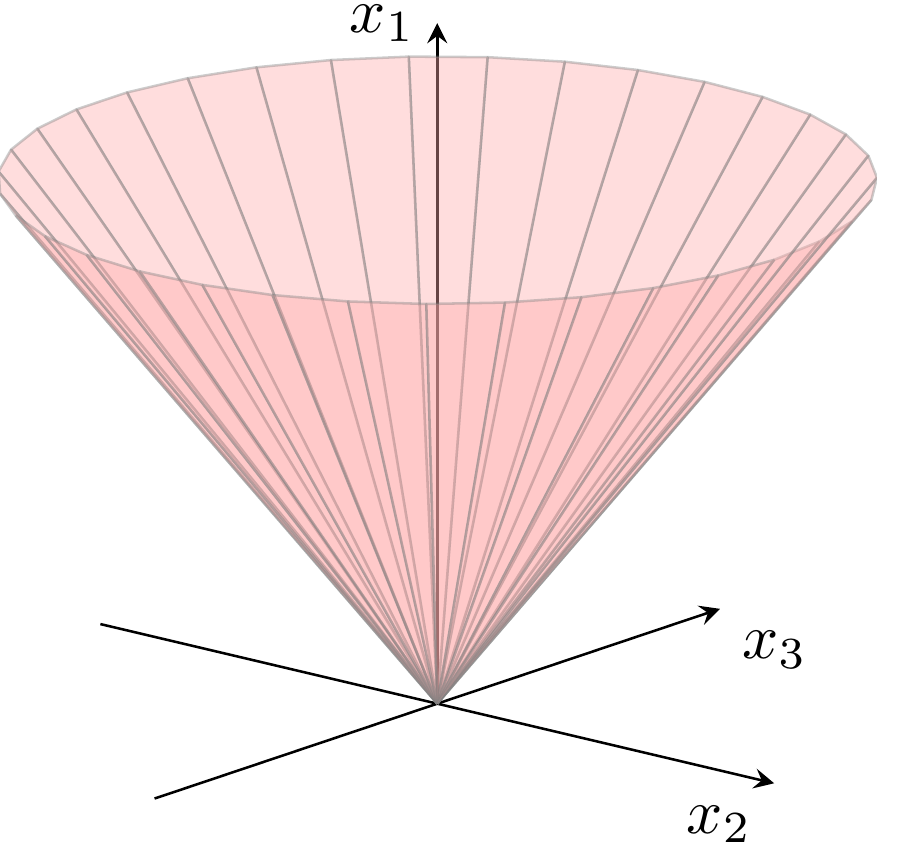
\includegraphics[width=0.4\textwidth]{../docs/Cone_Lorentz.png}
%             \caption{Mesh at exact interface}
%         \end{figure}
%     \end{overprint}
% \end{frame}